\documentclass[12pt, a4paper, twoside]{article}

\usepackage{blindtext}
\usepackage{geometry}
    \geometry{
        a4paper,
        total={170mm,257mm},
        left=20mm,
        top=20mm,
    }

%Paquetes   
\usepackage[utf8]{inputenc}
\usepackage[english]{babel}
\usepackage[table,xcdraw]{xcolor}
\usepackage{amsmath}
\usepackage{amsfonts}
\usepackage{amssymb}
\usepackage{graphicx}
\usepackage{multicol}
\usepackage{multirow}
\usepackage{changepage}
\usepackage{float}
% \usepackage{cite}
\usepackage{url}
\usepackage{indentfirst}
%%\usepackage{subfig}
\usepackage{subcaption}
\usepackage{enumerate}
\usepackage{circuitikz}
\usepackage{physics}
\usepackage{caption}
\usepackage{wrapfig}
%\usepackage{hyperref}
%\usepackage[colorlinks=true, linkcolor=Maroon, urlcolor=Maroon]{hyperref} %%SACAR BOXES ROJOS
\usepackage{bookmark}

\usepackage{amssymb} %simbolos matematicos especiales
\usepackage{csquotes}
\usepackage{bm}

\usepackage{MnSymbol}

%unidades
\usepackage{siunitx}

%figuras EPS
\usepackage{epsfig}

%quotes
\usepackage{csquotes}

% %bibiliography
\usepackage[backend=bibtex, style=numeric-comp, maxbibnames=5, sorting=none]{biblatex}%%bibliografía
\addbibresource{./biblio.bib}

%float package: ESPACIOS POR DEBAJO Y POR ENCIMA DE FIGURAS
\renewcommand{\topfraction}{0.85}
\renewcommand{\bottomfraction}{0.85}
\renewcommand{\textfraction}{0.15}
\renewcommand{\floatpagefraction}{0.8}
\renewcommand{\textfraction}{0.1}
\setlength{\floatsep}{5pt}
\setlength{\textfloatsep}{5pt plus 2pt minus 2pt}
\setlength{\intextsep}{5pt plus 2pt minus 2pt}

%SVG images 
\usepackage[inkscapearea=page]{svg}

%Tikz
\usepackage{pgfplots}
\pgfplotsset{compat = newest}
\usepackage{tikz}
\usetikzlibrary{circuits.logic.US, circuits.ee.IEC}

%simbolos Real e imaginario
\usepackage{physics}
% EJEMPLOS declaración de environment
% 
\newcounter{testexample}
\usepackage[most]{tcolorbox}
\usepackage{xparse}
\def\exampletext{Teorema} % If English

\NewDocumentEnvironment{example}{ O{} }
{
\colorlet{colexam}{white} % Global example color
\newtcolorbox[use counter=testexample]{testexamplebox}{%
    % Example Frame Start
    empty,% Empty previously set parameters
    skin=bicolor,   %ESTAS DOS LINEAS SON PARA EL COLOR DE FONDO
    colback=blue!5!white,
    sharp corners,
        frame style={%ESTO ES PARA QUITARLE EL MARCO
            color=blue!10!white,
        },
    title={\exampletext: #1},% use \thetcbcounter to access the testexample counter text
    % Attaching a box requires an overlay
    attach boxed title to top left,
    % Ensures proper line breaking in longer titles
    minipage boxed title,
    % (boxed title style requires an overlay)
    boxed title style={enhanced, colback = blue!60!white, size=minimal, toprule=0pt,top=4pt,left=5mm, right= 6mm,overlay={}},
    coltitle=colexam,fonttitle=\bfseries,
    before=\par\medskip\noindent,parbox=false, boxsep=0pt,left=5mm,right=5mm,top=2pt,breakable,pad at break=0mm,
    before upper=\csname @totalleftmargin\endcsname0pt, % Use instead of parbox=true. This ensures parskip is inherited by box.
    % Handles box when it exists on one page only
    overlay unbroken={\draw[colexam,line width=2pt] ([xshift=-0pt]title.north west) -- ([xshift=-0pt]frame.south west); },
    % Handles multipage box: first page
    overlay first={\draw[colexam,line width=2pt] ([xshift=-0pt]title.north west) -- ([xshift=-0pt]frame.south west); },
    % Handles multipage box: middle page
    overlay middle={\draw[colexam,line width=2pt] ([xshift=-0pt]frame.north west) -- ([xshift=-0pt]frame.south west); },
    % Handles multipage box: last page
    overlay last={\draw[colexam,line width=2pt] ([xshift=-0pt]frame.north west) -- ([xshift=-0pt]frame.south west); },%
    }
\begin{testexamplebox}}
{\end{testexamplebox}\endlist}


%DEFINICIÓN - environment
\usepackage{amsthm}
\usepackage{thmtools}
% \usepackage{tkz-fct} 

\declaretheoremstyle[%
spaceabove=6pt, spacebelow=6pt,
headfont=\normalfont\bfseries\color{blue!60!black}, headindent=\parindent,
notefont=\mdseries, notebraces={(}{)},
bodyfont=\normalfont,
postheadspace=0.5em]%
{def}
\declaretheorem[name=Definición, numbered=yes, style=def]{definition}

%TEOREMA - environment
\declaretheoremstyle[%
spaceabove=6pt, spacebelow=6pt,
headfont=\normalfont\bfseries\color{blue!60!black}, headindent=\parindent,
notefont=\mdseries, notebraces={(}{)},
bodyfont=\normalfont,
postheadspace=0.5em]%
{theo}
\declaretheorem[name=Teorema, numbered=yes, style=theo]{teorema}

%OBSERVACIÓN - environment
\declaretheoremstyle[%
    spaceabove=6pt, spacebelow=6pt,
    headfont=\normalfont\bfseries\color{red!80!black}, headindent=\parindent,
    notefont=\mdseries, notebraces={(}{)},
    bodyfont=\normalfont,
    postheadspace=0.5em
    ]%
    {obs}
    \declaretheorem[name=\underline{\# Observación}, numbered=no, style=obs]{obs}


%FORMATEO DE TITULOS Y SECCIONES
\usepackage{titlesec}
\titleformat{\section} %qué tipo de comando
    [display]  %shape
    {\Large\bfseries\itshape} %estilo
    {} %algun texto o label
    {-1.5em} %separación
    {
        \centering
    }
    [
    \centering
    \vspace{-0.75ex}%
    \rule{\textwidth}{0.3pt}
    ] % after-code


    \titleformat{\subsection} %qué tipo de comando
    %[display]  %shape
    {\bfseries\itshape} %estilo
    {\thesubsection} %algun texto o label
    {0em} %separación
    {
    }
    [
        %\centering
        \vspace{-0.5ex}%
        \rule{\textwidth}{0.3pt}
    ] % after-code

%%%%%%%%%%%%%%%%%%%%%%%%%%%%%%%%%%%%%%%%%

%Listado Fancy
\usepackage{xcolor,enumitem,amssymb}
\let\svitem\item
\let\thebang\relax
\colorlet{bangcolor}{blue!30}
\newenvironment{bangenumerate}
{%
  \fboxsep=3pt\relax%
  \renewcommand\item[2][\relax]{%
    \ifx!##2%
      \def\thebang{\makebox[0pt][l]{\kern-1pt\textcolor{bangcolor}{%
        \raisebox{1pt}{$\scriptstyle\blacktriangleright$}}}}%
      \def\next{}%
    \else%
      \def\thebang{}%
      \def\next{##2}%
    \fi%
    \ifx\relax##1\relax\svitem\else\svitem[##1]\fi\next%
  }%
  \begin{enumerate}[label={%
    \smash{\colorbox{bangcolor}{\bfseries\sffamily\theenumi)}\thebang}}]%
}{\end{enumerate}}

%%Change table of contents title!!
\renewcommand{\contentsname}{Contenidos}

\renewcommand{\figurename}{Figura}


%%%%%%%%%%%%%%%%%%%%%%%%%

\begin{document}
    \thispagestyle{empty}
        %encabezado
        \pagestyle{plain}{
        \pagestyle{empty}
        \changepage{3cm}{1cm}{-0.5cm}{-0.5cm}{}{-2cm}{}{}{}
        \noindent
        {\small
            \begin{center}
            \begin{tabular}{c}
                
\includegraphics[width=7cm]{imagenes/uns_logo.jpg}
            \end{tabular}
            \end{center}
        }
        \vspace{0.5cm}
        %-------------------Datos de la carátula
        \begin{center}
            \par %espacio antes del encabezado
            {
                \Huge{
                   Universidad Nacional del Sur
                }   
            }
            \par\vspace{0.1cm}
            {
                \large{}
            }
            \par\vspace{8cm}
            {
                \Large\textbf{Proyecto Final de Carrera}
            }

            \par\vspace{0.2cm}
            {
                \Large{Implementación de un conversor tiempo a digital en FPGA.}
            }
            \par\vspace{0.4cm}
            
            %    \large\textbf{1° Cuatrimestre 2021}
            
            %%\par\vspace{10cm}
        \end{center}
        }
        \begin{center}
            
            \par\hspace{1cm}
            {
            \large Autor: Filsinger, Miqueas\\
            \vspace*{0.5cm}%
            \large Director: Morales, Juan Ignacio \\
            \large Codirector: Paolini, Eduardo            
            }  
        \end{center}
            
        \clearpage
        
    \tableofcontents
    \newpage
    \clearpage

\section{Introducción}
Un TDC (Time to Digital Converter) es un circuito electrónico capaz de medir un intervalo de tiempo con alta precisión y convertirlo en un valor digital. 
Fueron impulsados principalmente en el campo de la física atómica y de altas energías \cite{Altruda2023}, radares tipo LiDAR \cite{Maatta1998}, 
y aplicaciones biomédicas como tomografías por emisión de positrones (PET). Estas distintas aplicaciones normalmente utilizan  ASICs off-the-shelf para
implementarlo; sin embargo los recientes avances tecnológicos en FPGA han permitido realizar diseños
que alcanzan una precisión temporal del orden de los pocos picosegundos, contando con la ventaja de ser flexibles y la posibilidad de integrar la aplicación
en un único dispositivo. \\

Particularmente, en \cite{Nacho} se diseñó y fabricó 
un chip que implementa cadenas de retardo programables, donde el elemento de retardo se basa
en un inversor CMOS que mediante un registro de configuración puede añadir capacidades a su 
salida (SCI) o modificar su resistencia equivalente (CSI), como muestra la Figura \ref{fig: nacho_delay}.
Esta configuración permite la posterior ecualización de la cadena de retardos, celda a celda,
siendo el retardo promedio configurable de $\tau ' = 65$ps.
En este trabajo se explora la posibilidad de replicar y mejorar dicha precisión dentro de una FPGA,
con el fin de poder obtener idealmente varias muestras en el orden de las decenas de picosegundos, 
de modo que se logre una ecualización aproximada de la cadena de retardos.

\begin{figure}[H]
      \centering
      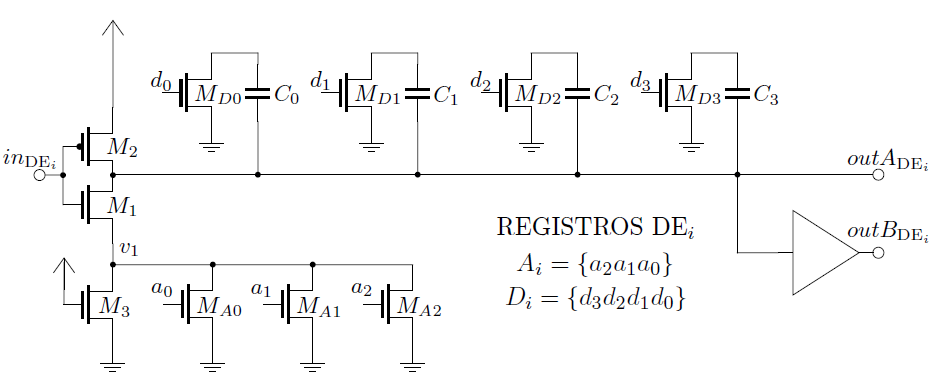
\includegraphics[width=0.75\textwidth]{imagenes/nacho_delay.png}
      \caption{Esquemático circuital del elemento de retardo.}
      \label{fig: nacho_delay}
\end{figure}

El enfoque se centra en maximizar la precisión y la linealidad, dos de los principales criterios de rendimiento de un TDC.
La precisión se refiere a la mínima unidad que el instrumento es capaz de medir, mientras que el concepto de linealidad refiere
a la capacidad de mantener la respuesta entrada-salida proporcional en todo el rango de trabajo. 
Son interesantes además algunos
otros aspectos como el rango de medición, el tiempo muerto, su consumo de energía, y la frecuencia de muestreo,
sin embargo se omitieron en este trabajo.\\

\clearpage





\section{Estado del arte}
En esta sección se explicarán algunos de los últimos avances propuestos en la bibliografía. Hasta ahora se ha hablado de
aquellos aspectos esperables en un TDC, pero es importante tener en cuenta que existen distintos paradigmas en su diseño dependiendo
de su destino: ASIC o FPGA. La libertad en la colocación de componentes (placement \& routing) 
en el diseño de ASICs permite minimizar retardos indeseados, algo que resulta desafiante en el diseño de FPGAs. Por esta razón,
se basa en gran medida en \cite{Machado} ya que propone un estudio, clasificación y análisis de las distintas 
arquitecturas específicamente orientadas a FPGA, algo que no se había hecho hasta el momento.\\

Machado propone clasificar las distintas arquitecturas según los componentes que utiliza, de esta forma propone la taxonomía que
se muestra en la Figura \ref{fig: taxonomia}.
\begin{figure}[H]
     \centering
     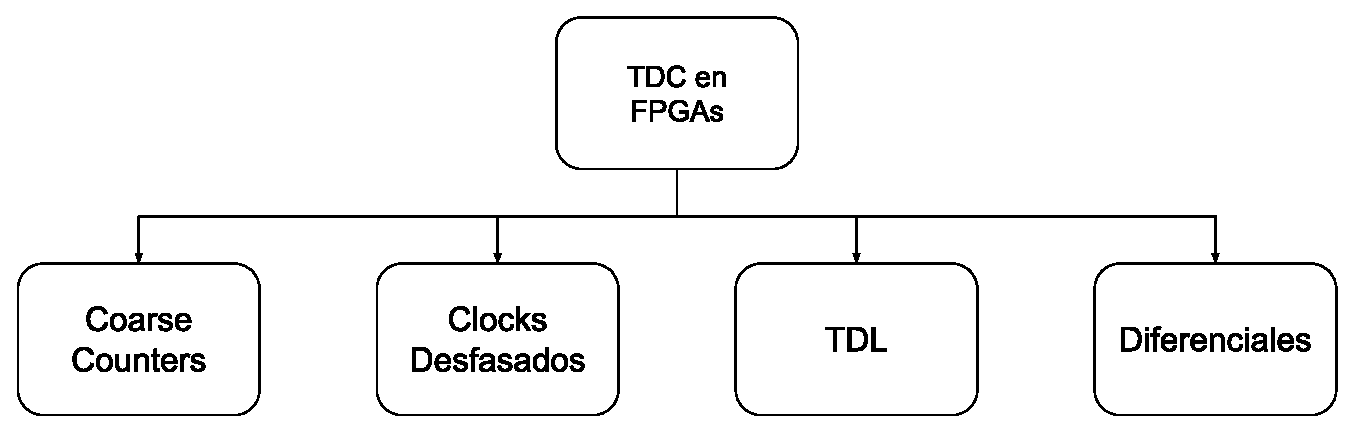
\includegraphics[width=0.75\textwidth]{imagenes/taxonomia.eps}
     \caption{Clasificación de las distintas arquitecturas.}
     \label{fig: taxonomia}
\end{figure}
Las arquitecturas de tipo \textit{Coarse Counter} (contador grueso), son aquellas que utilizan 
un simple contador para estimar el ancho de pulso de una señal, según la cantidad de clocks del 
sistema que entran en ella; su precisión es entonces el período de reloj. Las arquitecturas basadas 
en \textit{Relojes Desfasados} son todas aquellas que utilizan más de un clock para estimar la medición:
algunas de ellas deciden la medición a partir de saber cuál clock puede observar primero la llegada del pulso, 
mientras que otros utilizan elementos adicionales para la interpolación. 
Por otro lado está tal vez una de las arquitecturas más utilizadas, aplicada en este trabajo, y es aquella 
que utiliza \textit{Tapped Delay Lines} (TDL: lineas de retardo) para realizar la interpolación y 
generar la medición fina. Esto es, se ingresa el pulso de entrada en una cadena de elementos que introducen un 
retardo uniforme; al muestrear el estado de la cadena entonces se infiere cuántos retardos la señal cruzó, con lo 
que se estima una medición. Dentro de esta clasificación existen distintas formas de utilizar esta forma de 
interpolación, algunas arquitecturas extienden el rango de medición al combinar también un Coarse Counter (la
topología Nutt) otras utilizan varias cadenas de retardo con el fin de mejorar la precisión realizando un 
promedio de ellas, y otras combinan más de una cadena y más de un clock. En cualquiera de sus formas, se 
clasifican según su componente principal de interpolación:
la cadena de retardos. Por último, las arquitecturas \textit{Diferenciales} se basan en medir la diferencia 
de retardo entre dos elementos. En estas existen principalmente dos tipos: cadenas de retardos compuestas de 
dos elementos de retardo distintos, y osciladores en anillo.
Por otro lado si buscamos medir el intervalo temporal entre una señal y el clock entonces llamaremos al TDC 
\textit{síncrono}, si el intervalo puede comenzar y terminar en cualquier momento entonces lo llamaremos 
\textit{asíncrono}.\\

\subsection{Principios de la arquitectura tipo Nutt}
Las arquitecturas TDL pueden ser implementadas de distintas formas, como muestra la Figura \ref{fig: various_tdl}.
\begin{figure}[H]
     \centering
     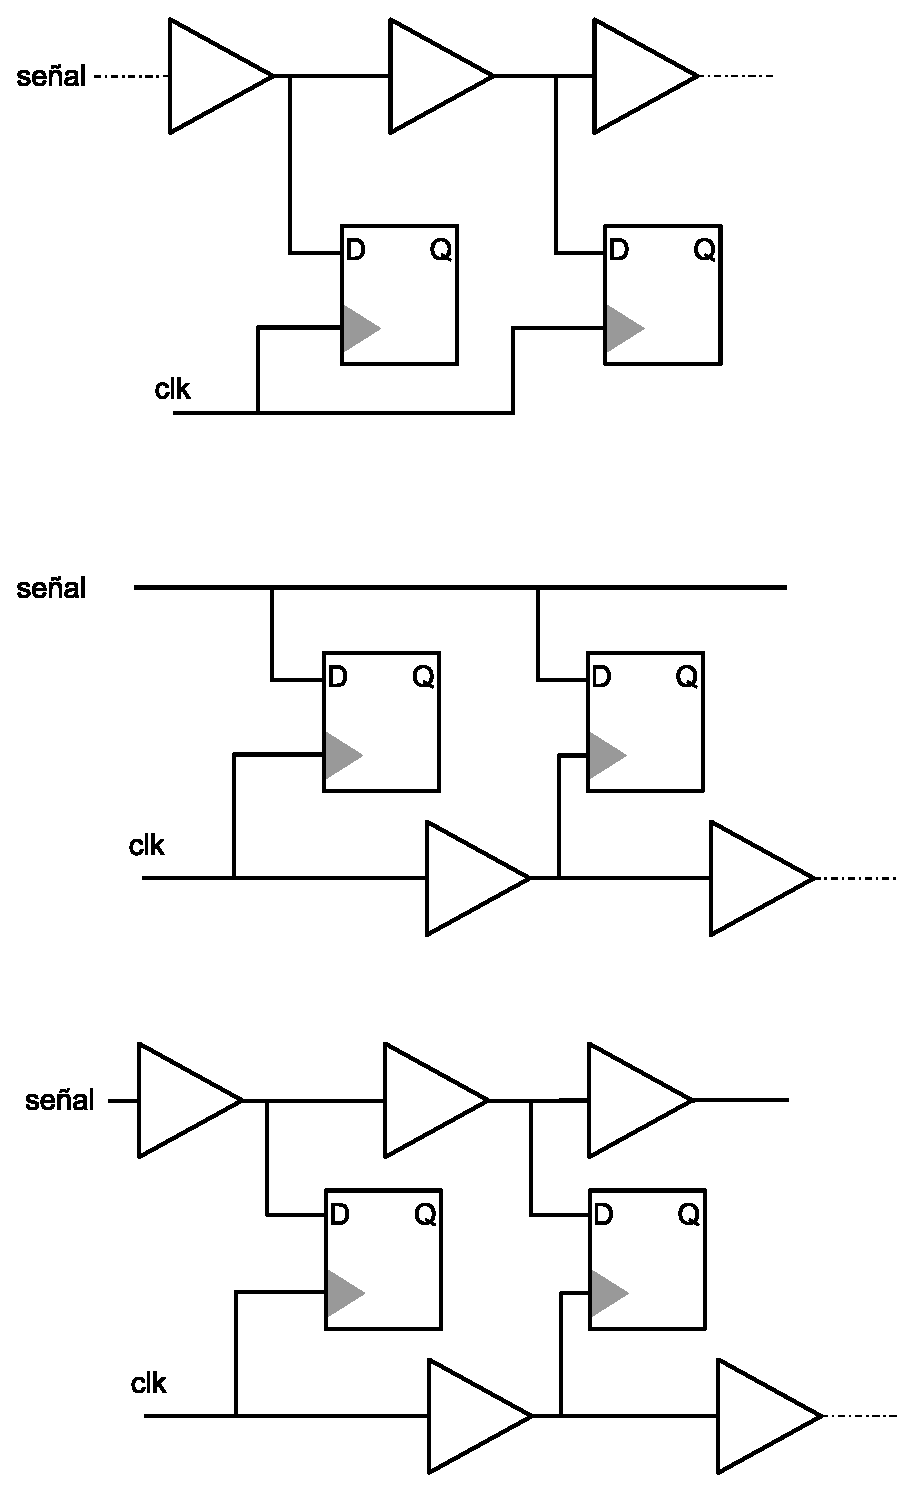
\includegraphics[width=0.75\textwidth]{imagenes/various_tdl.eps}
     \caption{Diferentes formas de aplicar el método Vernier.}
     \label{fig: various_tdl}
\end{figure}
El último diseño presentada en la figura representa un TDC Diferencial, donde la
idea principal es utilizar unidades de retardo distinto tal que se pueda calcular
el tiempo fino como $t_\text{fino} = n \cdot (\tau_1 - \tau_2)$. A diferencia 
del diseño en ASIC, en FPGA es difícil
tener muchas celdas con distintos retardos, por lo que usualmente se implementa la misma celda
y luego se agrega un retardo por ruteo, pero esto es tan poco uniforme y controlable que 
hace que esta opción sea poco implementable. Por otro lado, el segundo diseño es en esencia igual al primero,
sin embargo los fabricantes ponen un esfuerzo enorme en poder generar ruteos
de reloj precisos, con el mínimo desfase posible. Intentar intervenir el ruteo de reloj en una FPGA
carece de sentido. Específicamente se utilizó la primer opción, donde la señal alimenta una cadena de retardos, 
la cual se registra a cada reloj. Cuando se detecta la entrada de un pulso, se genera una señal de \textit{Start}, y
el valor de la cadena de flip flops se guarda para luego ser procesado, representando el valor entre líneas
rojas en la Figura \ref{fig: arqui_tdl}. Cuando la señal egresa de la cadena de retardos, se genera la señal
 de \textit{Stop}, con la que se vuelve a registrar el valor de la cadena. Finalmente, tal como implementa la
topología Nutt, el resultado se compone de una parte gruesa y una parte fina, y puede calcularse como:
\begin{equation*}
     T_{m} = N_{coarse} \; T + \tau_{start} - \tau_{stop}
\end{equation*}

\begin{figure}[H]
     \centering
     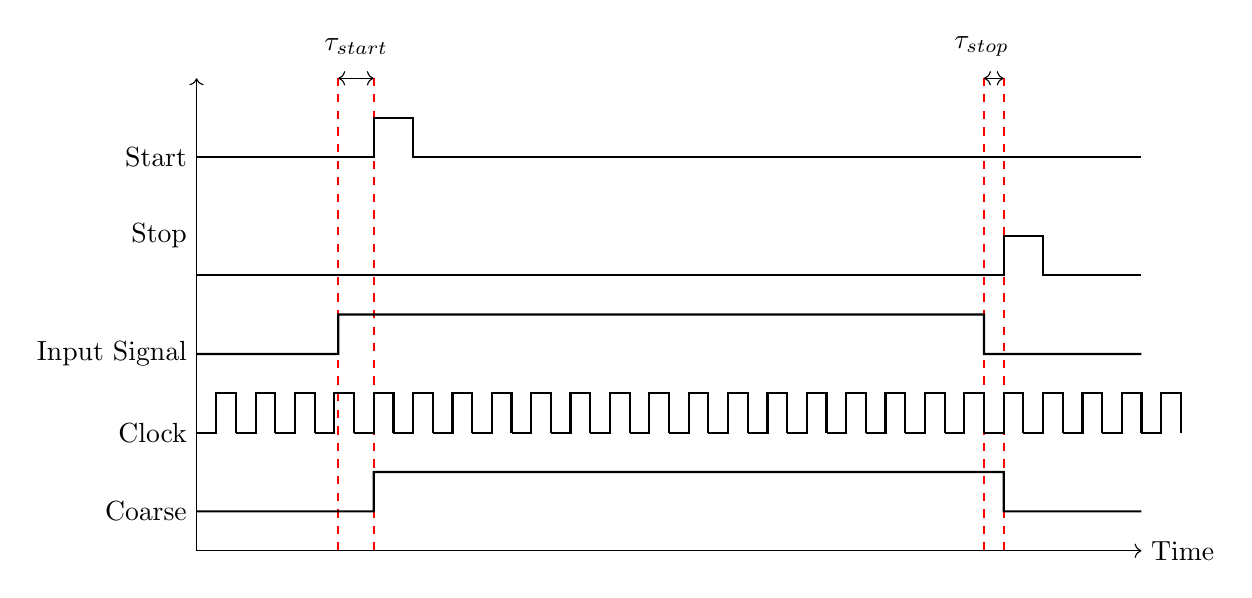
\begin{tikzpicture}
          % Define styles
          \tikzstyle{signal} = [thick]
          \tikzstyle{startstop} = [red, thick, dashed]

          % Dashed lines for START and STOP
          \draw[startstop]    (1.8,0)   -- (1.8,6);
          \draw[startstop]    (2.25,0)  -- (2.25,6);
          \draw[startstop]    (10,0)    -- (10,6);
          \draw[startstop]    (10.25,0) -- (10.25,6);

          %Cotas
          \draw[<->]          (1.8, 6)  -- (2.25, 6);
          \node[right] at (1.5, 6.4) {$\tau_{start}$};
          \draw[<->]          (10, 6)  -- (10.25, 6);
          \node[right] at (9.5, 6.4) {$\tau_{stop}$};

          % Time axis
          \draw[->] (0,0) -- (12,0) node[right] {Time};

          % START signal
          \draw[signal] (0,5) -- ++(2.25, 0) -- ++(0, 0.5) -- ++(0.5, 0) -- ++(0, -0.5) -- (12,5);
          \node[left] at (0,5) {Start};

          % STOP signal
          \draw[signal] (0,3.5) -- (10.25,3.5) -- (10.25,4) -- (10.75, 4) -- (10.75, 3.5) -- (12,3.5);
          \node[left] at (0,4) {Stop};

          %%Input signal
          \draw[signal] (0,2.5) -- ++(1.8,0) -- ++(0,0.5) -- (10,3) -- ++(0,-0.5) -- (12,2.5);
          \node[left] at (0,2.5) {Input Signal};

          % Clock signal
          \foreach \x in {0,0.5,...,12} {
               \draw[signal] (\x, 1.5) -- ++(0.25, 0) -- ++(0, 0.5) -- ++(0.25, 0) -- ++(0,-0.5);
          }
          \node[left] at (0,1.5) {Clock};

          %%Coarse signal
          \draw[signal] (0,0.5) -- ++(2.25,0) -- ++(0,0.5) -- (10.25,1) -- ++(0,-0.5) -- (12,0.5);
          \node[left] at (0,0.5) {Coarse};

          % Extra line to mark the end
          \draw[<-] (0,6) -- (0, 0);

     \end{tikzpicture}
      \caption{Esquema de medición fina de un Nutt-TDC.}
      \label{fig: arqui_tdl}
\end{figure}

\subsection{Tests, mediciones y resultados}
Particularmente en la arquitectura TDL, la opción predilecta en la bibliografía para calibrar el instrumento es mediante 
un prueba de densidad de código o ``code-density test''. Esta prueba consiste en ingresar una señal decorrelacionada del reloj del sistema, de forma que 
excite todos los elementos de retardo por igual y por lo tanto ``golpee'' a cada celda en función de su retardo real.
Una celda con un retardo más grande será detectada más veces. 
Si la cadena tiene $N_c$ elementos, mide un período de reloj $T$, se realiza el test con $N$ muestras,
y la i-ésima celda captura $n_i$ mediciones entonces es claro que el 
tamaño de cada retardo es
\begin{equation}
     \tau_i = n_i \; \dfrac{T}{N} \; ,
     \label{eq: tau_i}
\end{equation}
y el retardo medio, es decir el retardo de cada celda si es equiprobable obtener un hit 
en cada bin, es
\begin{equation}
     \hat{\tau} = \dfrac{T}{N_c} \; .
     \label{eq: tau_medio}
\end{equation}
La explicación de esto es que a medida que la cadena se acerca a una cadena ideal, la probabilidad de golpear cada
elemento debe ser la misma para todos los elementos y es la cantidad de veces que se obtiene un hit
sobre la cantidad de experimentos totales, esto es $n_i/N$. Para una cantidad de mediciones grande,
esta probabilidad debe acercarse a $1/N_c$. Al igual que lanzar un dado no cargado, como es
equiprobable obtener cualquiera de sus seis caras entonces la ley de grandes números nos dice
que para una cantidad suficientemente grande de experimentos, deberíamos obtener cada cara una misma cantidad
de veces, esto es que cada cara salga $1/6$ de las veces que se arroja el dado.
Entonces, en el TDC debe ocurrir que 
\begin{equation*}
     \dfrac{n_i}{N} \longrightarrow \dfrac{1}{N_c} \; ,
\end{equation*}
que es equivalente a que $\tau_i \longrightarrow \hat{\tau}$, a medida que $N \rightarrow \infty$.
Con esto es posible calcular las no linealidades de cada bin tomando como referencia
el tiempo ideal $\hat{\tau}$. La no linealidad diferencial DNL (Differential Non-Linearity) 
se puede calcular como
\begin{equation}
     DNL_i = \tau_i - \hat{\tau} \; ,
     \label{eq: DNL}
\end{equation}
y con esto la no linealidad integral INL (Integral Non-Linearity), es decir las no linealidades acumuladas a medida que la 
señal atraviesa la cadena, como
\begin{equation}
     INL_i = \sum_{j=0}^{i-1} {\tau_j - \hat{\tau}} \; .
     \label{eq: INL}
\end{equation}

Para obtener la DNL en función del bit menos significativo (LSB), poniendo 
en evidencia cuántos bits de incertidumbre representa cada no linealidad, 
se puede normalizar la no linealidad en segundos por el retardo medio tal que $DNL_i[LSB] = DNL_i[\rm{s}] / \hat{\tau}$.\\
Conociendo estas propiedades es posible generar una ``tabla de calibración''. Una vez que el TDC
finaliza la medición del ancho de pulso, se corrige mediante una tabla pre-cargada en memoria, entregando un resultado
calibrado al instante de medición (on-line calibration \cite{Liu2015}). Se puede contemplar
una calibración exclusiva para el flanco \textit{Start} y otra para el flanco \textit{Stop} (\cite{Khaddour2023}), y 
corregir variaciones en las condiciones PVT\footnote{Proceso, voltaje, y temperatura.} (\cite{Qin2017}).
Con esto, es posible corregir limitaciones de diseño y hardware mediante una buena calibración.\\

\section{Arquitectura}

A este tipo de estructuras digitales nos gusta llamarlas \textit{ad-hoc}, ya que desde su concepción hasta su
implementación podremos ver que no se puede enmarcar dentro de una estructura típica, sino que su diseño viene estrechamente ligado
a su aplicación en particular. A simple vista puede verse que los elementos que se utilizarán, las etapas de procesamiento,
y las técnicas implementadas son poco comunes para lo que es el mundo del diseño digital. Se da a continuación 
una explicación descriptiva de cada bloque fundamental que conforma la arquitectura del \textit{TDC}.

\subsection{Tapped Delay Line}
El bloque principal de este diseño, encargado de realizar la \textit{medición fina}, es una cadena de retardos.
Para implementar estos retardos existen opciones distintas pero acotadas para una implementación en FPGA. En sus
inicios la solución predilecta era utilizar multiplexores en cadena \cite{kalisz_field-programmable-gate-array-based_1997},
pero para aprovechar las ventajas propias de la estructura de una FPGA se evolucionó a utilizar
\textit{Carry4s}, posiblemente utilizado por primera vez en \cite{favi_17ps_2009}. Estos elementos
forman parte de la unidad mínima de trabajo en una FPGA, y su combinación con LUTs, flip flops, y Multiplexores forman lo que 
se conoce como un \textit{SLICE}\footnote[1]{La Artix-7 cuenta con un total de 33650 slices.}. 
Los \textit{Carry4s} en su concepción fueron destinados para implementar sumadores, y tienen la ventaja de estar optimizados
para tener el mínimo retardo entre compuerta y compuerta. Además cada salida cuenta con un flip flop routeado inmediatamente
a continuación, como se muestra en la Figura \ref{SliceYCarry}.

\begin{figure}[H]
     \centering
     \begin{subfigure}{0.45\textwidth}
           \centering
           \resizebox{\linewidth}{!}{
           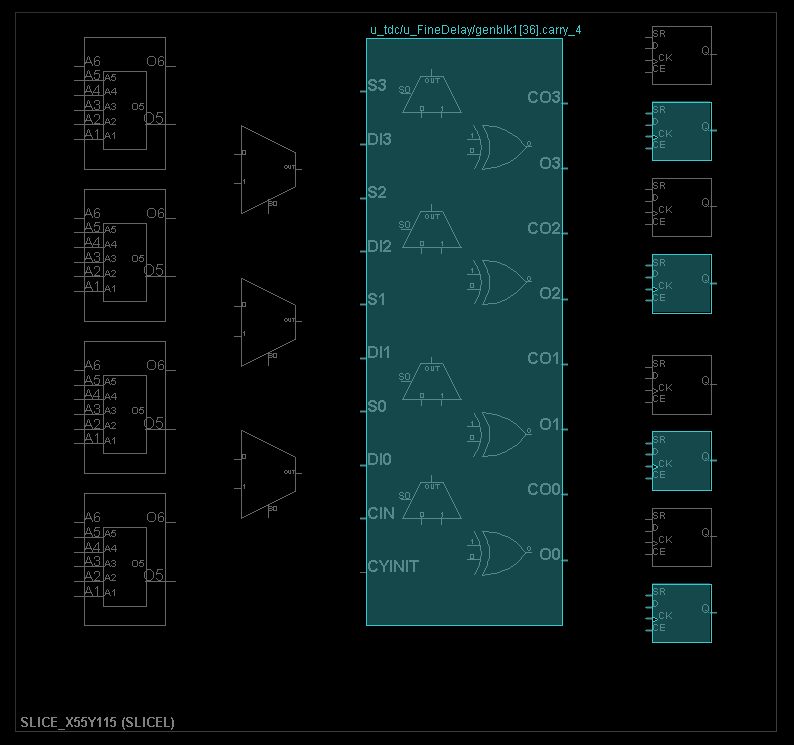
\includegraphics[]{imagenes/slice.png}
           }
           \caption{SLICE L de una Artix-7 en Vivado 2023.2}
     \end{subfigure}%
     \hspace{10pt}%
     \begin{subfigure}{0.4\textwidth}
           \centering
           \resizebox{\linewidth}{!}{
           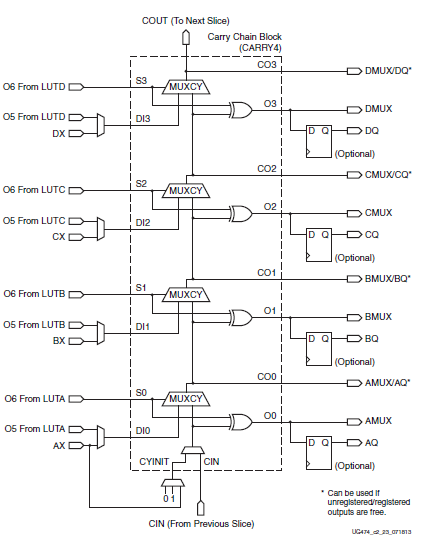
\includegraphics[]{imagenes/carry4.png}
           }
           \caption{Carry 4}
     \end{subfigure}
     \caption{Elementos disponibles dentro de una SLICE.}
     \label{SliceYCarry}
\end{figure}%

Cada Carry4 cuenta con 4 salidas que pasan por una XOR, (O0-O3) y 4 salidas que pasan por
cada MUXCY (CO0-CO3), además cuenta con un puerto \textit{CIN} con el propósito de colocarlas
en cadena y una entrada auxiliar \textit{CYINIT} desde donde ingresará el pulso externo.\\
Como la implementación aquí presentada es asíncrona precisamos capturar la señal en su flanco de entrada y de
salida de la cadena de retardos, por lo que luego de la colocación de la primer columna de flip flops (\textit{First} flip flops) 
como se ve en \ref{SliceYCarry}, se utilizan otras dos columnas de flip flops llamados \textit{Start} flip flops y \textit{Stop} 
flip flops. Estos se encargan de registrar la primer columna solamente cuando se detecta un flanco de subida o de bajada,
a través de su \textit{Clock Enable}. Así se genera la estructura que se ve a continuación en la Figura \ref{fig: fine}.

\begin{figure}[H]
     \centering
     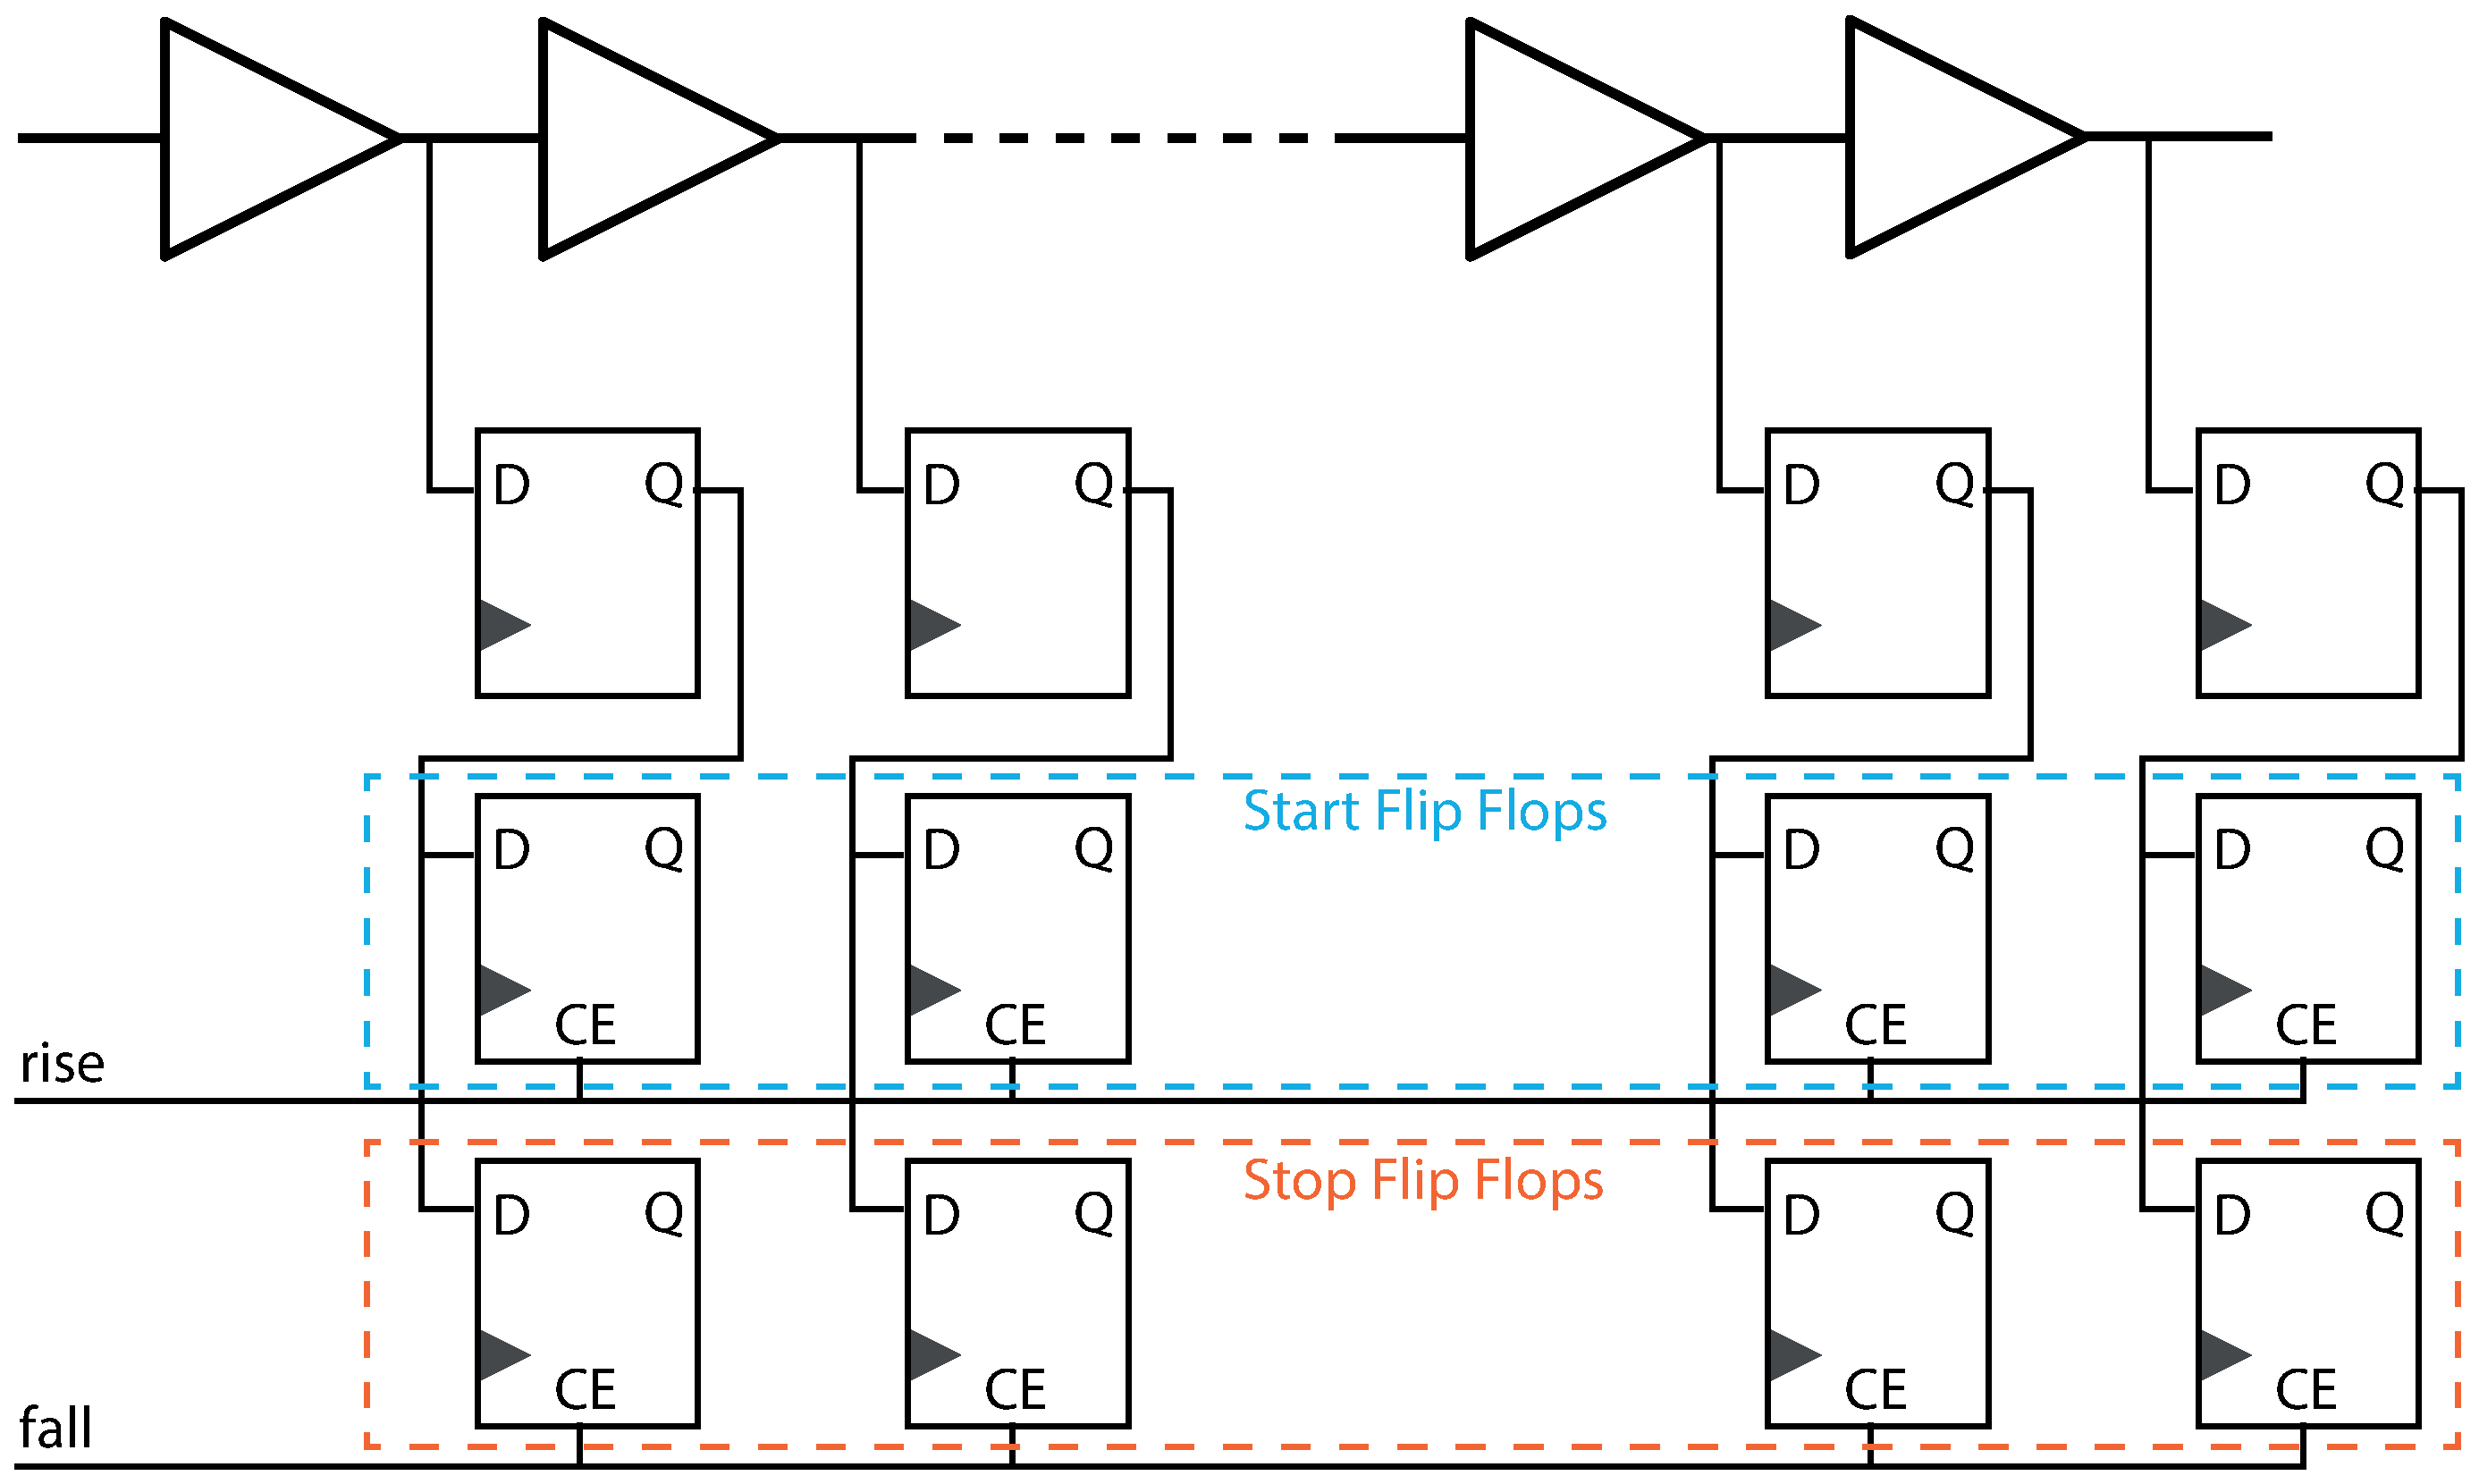
\includegraphics[width=0.7\textwidth]{imagenes/fine.eps}
     \caption{Esquema de la cadena del módulo de interpolación fina.}
     \label{fig: fine}
\end{figure}

De esta estructura surgen dos aspectos importantes:
\begin{bangenumerate}
     \item Es sabido que la transferencia de información análoga a digital puede producir metastabilidades si no se 
     realiza correctamente. La configuración de doble flip flop para registrar los elementos de retardo soluciona
     este problema introduciendo lo que se conoce como ``sincronizador''. \\
     Esto es, si el tiempo de establecimiento de la señal
     externa es menor al tiempo de establecimiento requerido por un sólo flip flop, este puede obtener
     un valor desconocido a la salida. Sin embargo introduciendo un segundo flip flop en serie, este no sufre
     de este problema, ya que en el próximo clock la señal es estable, y esta indeterminación se resuelve
     decantando hacia un estado. Además la técnica de doble registro reduce los problemas de burbujas
     en el resultado \cite{machado_novel_2018}.

     \item Una propiedad intrínseca del diseño tipo Nutt es que el ancho de pulso a medir
     debe ser al menos de un periodo de reloj. Esta es una condición de diseño
     y se aprovecha en múltiples bloques, pero en particular aquí
     se puede ver que el registro de \textit{Start} y \textit{Stop} dependen de un flanco de subida o bajada para
     generar la señal de \textit{Clock Enable}, la cuál tiene una duración de un reloj.
\end{bangenumerate}

%%%%TODO: revisar lo siguiente!
Por otro lado, es importante prestar especial atención al ruteo y colocación de cada elemento en la implementación final,
pues es preponderante en la calidad de los resultados del TDC. Si los retardos introducidos por el ruteo son 
uniformes para cada elemento de retardo entonces podemos asegurar que la calibración es capaz de corregir
en gran parte estos errores. Según \cite{machado_novel_2018} es importante colocar la cadena de retardos en las Slices
que quedan a continuación de los buffers de reloj, y que los flip flops sean colocados también cerca de la cadena. Esto
fue probado empíricamente y se obtuvieron mejores resultados cuando los extremos de la cadena de retardos quedaban simétricos
respecto de los clock buffers.\\
Experimentalmente se observó que cuando el extremo inferior de la cadena es lejano a los buffers, 
se pueden observar huecos en el histograma resultante, mientras que al colocarlo simétrico, este espacio
se reparte al inicio y al final de la cadena, como se ilustra en la Figura \ref{fig: problema buffer}.

\begin{figure}[H]
     \centering
     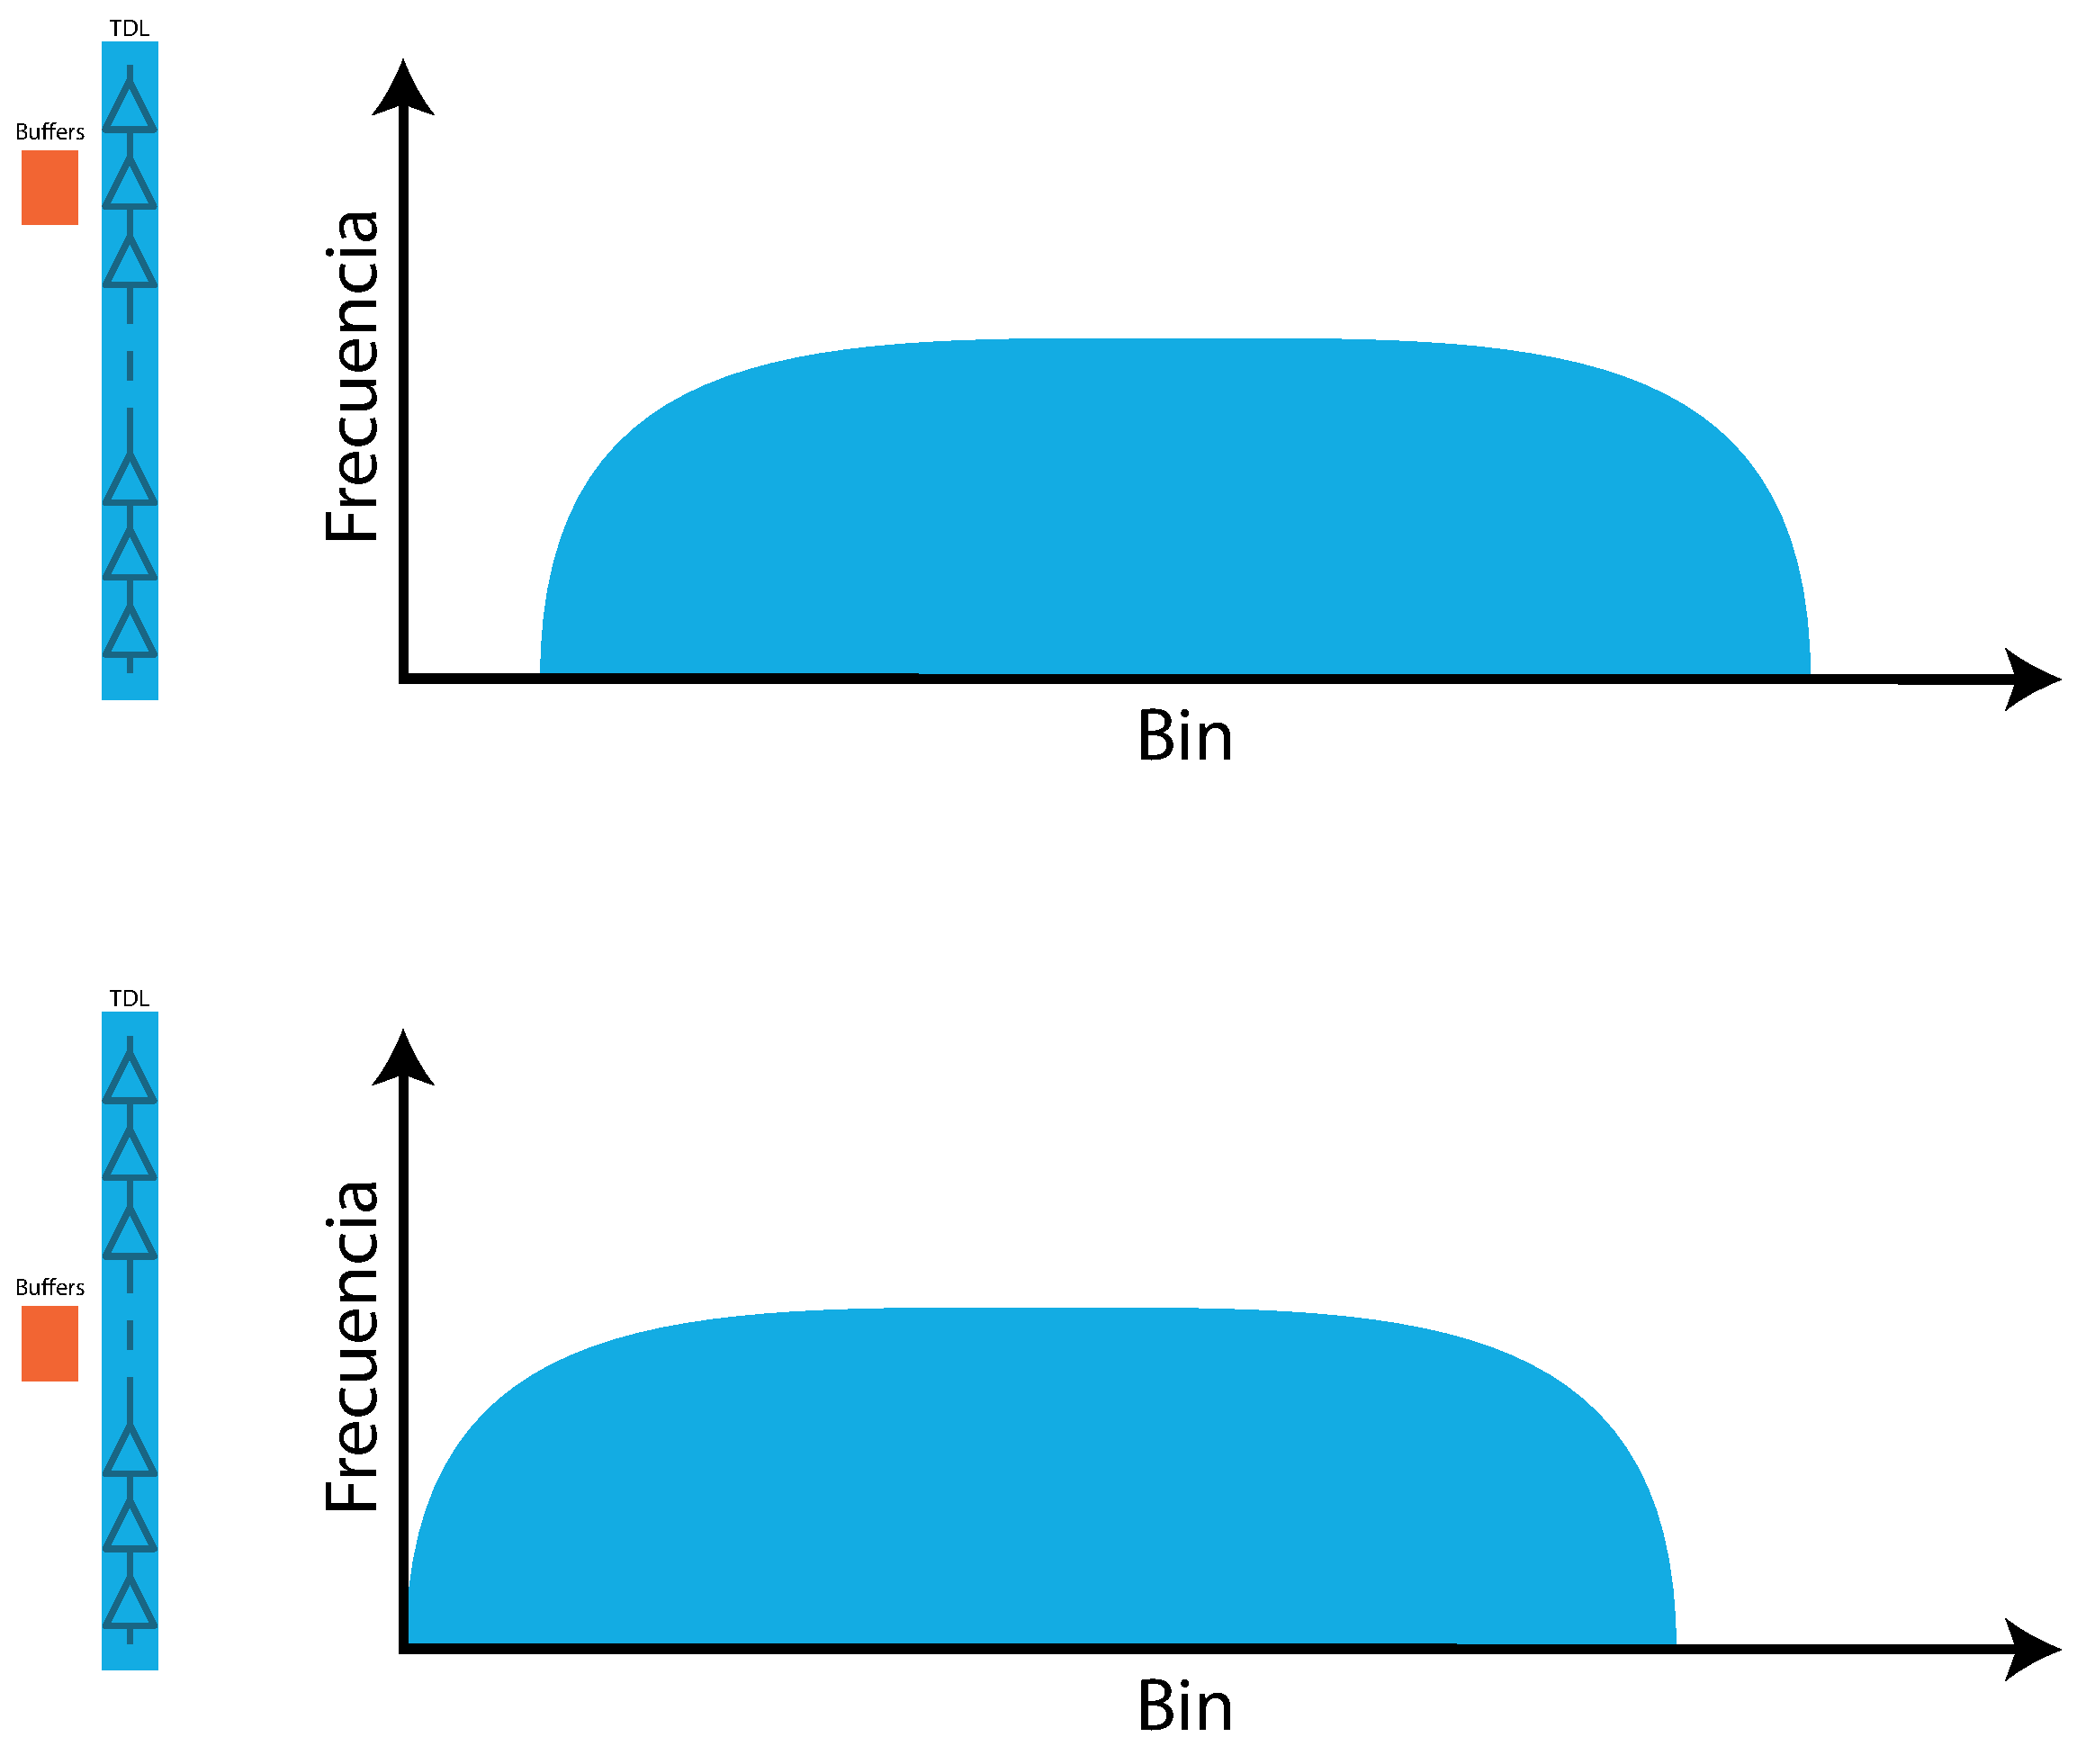
\includegraphics[width=0.75\textwidth]{imagenes/problema_buffer.eps}
     \caption{Ejemplo de histograma conseguidos al excitar el TDC con una frecuencia pseudo-aleatoria 
     modificando la posición relativa de la cadena de retardos respecto a los buffers de reloj.}
     \label{fig: problema buffer}
\end{figure}

\subsection{Decodificador}
La propagación de un pulso por la línea de retardos naturalmente genera un código unario sobre los 
registros. Esto es, a medida que el flanco descendente progresa sobre la línea de retardos deja a 
su paso un estado alto en cada flip flop de la cadena, mientra que cuando egresa un flanco ascendente 
deja ceros a su paso, tal como muestra la Figura \ref{fig: tdl_flancos}.

\begin{figure}[H]
     \centering
     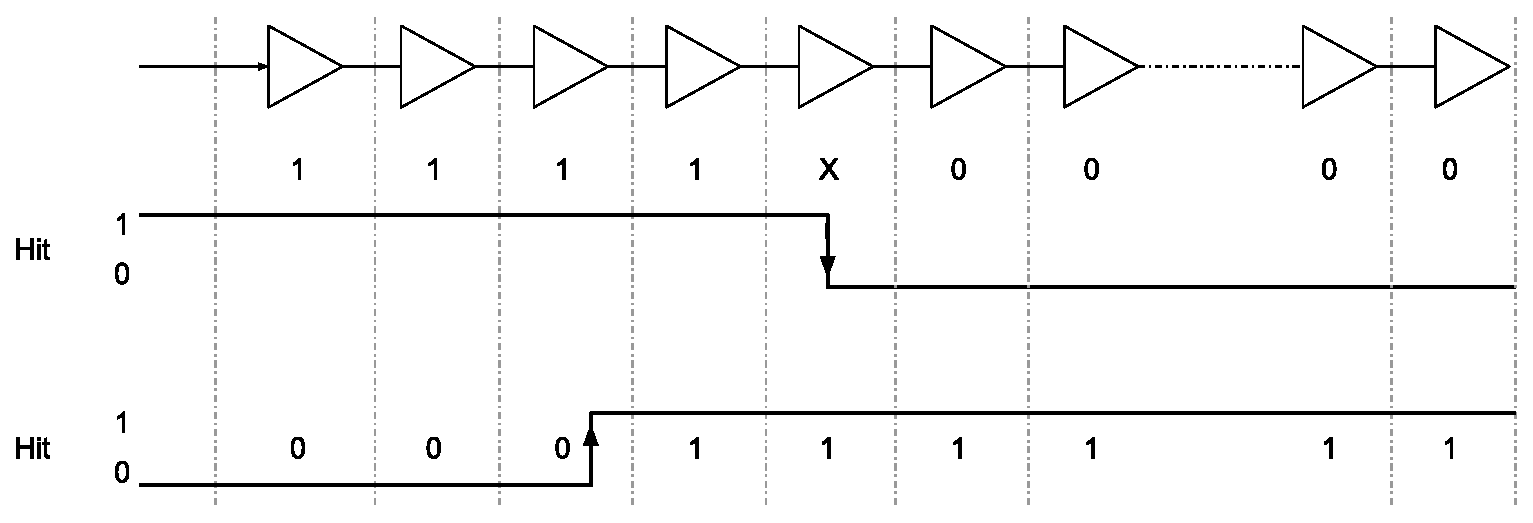
\includegraphics[width=0.75\textwidth]{imagenes/tdl_flancos.eps}
     \caption{Registro de un pulso digital en el momento que ingresa a la línea, y en el momento
     que egresa de ella.}
     \label{fig: tdl_flancos}
\end{figure}

La misión principal del decodificador es traducir estos valores leídos de los registros \textit{Start} y \textit{Stop} a datos procesables. 
Aquí se presenta un gran inconveniente en todas las soluciones propuestas por la bibliografía, pues debido a las variabilidades
propias de la arquitectura de una FPGA y de los órdenes de precisión que se pretenden es muy frecuente encontrar burbujas en los registros
resultantes, imposibilitando la utilización de decodificadores unarios convencionales. Esto significa que en los registros \textit{Start} o
\textit{Stop} se pueden encontrar registros con errores del tipo ``11..111001000...'', donde no es posible distinguir una transición de
estados clara. Según la bibliografía (\cite{Machado}) esto se debe principalmente al efecto de desfase de reloj (\textit{clock skew})
cada vez más presente en los últimas tecnologías, gracias al decrecimiento abrupto de tamaño de fabricación. Es posible que la diferencia 
temporal del flanco de clock (debido al desfase) 
entre dos flip flops que registran elementos de retardo adyacentes sea mayor al tiempo de retardo de la celda a registrar, y por lo tanto 
se produce una burbuja en el registro. Esto se ejemplifica en la Figura \ref{fig: bubble}. Si el flip flop número uno
captura la cadena en el momento $t_1$ y el flip flop número dos lo hace un momento después en $t_2$, es posible entonces que el primero
decante su estado en un valor $0$, mientras que el segundo decante su estado en un valor $1$ si $\Delta = t_2 - t_1 \geq \tau$
siendo $\tau$ el tiempo de una celda de retardo, y $\Delta$ el desfase entre relojes.

\begin{figure}[H]
      \centering
      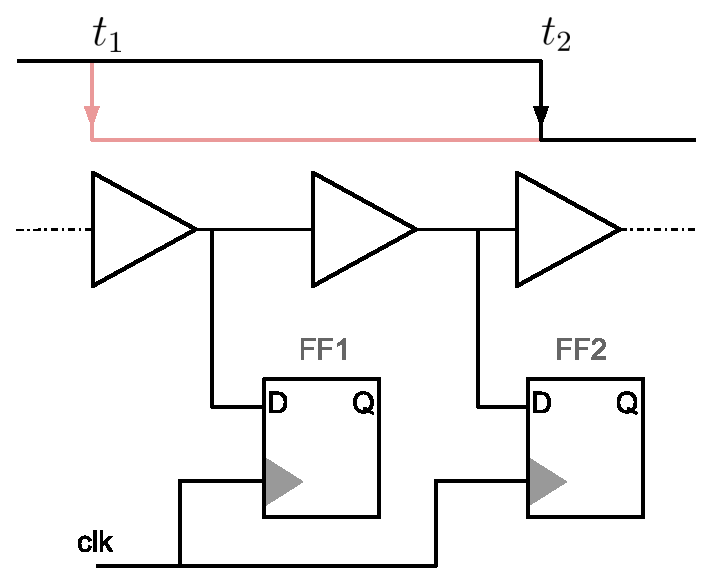
\includegraphics[width=0.55\textwidth]{imagenes/bubble.eps}
      \caption{Retardo virtual de propagación que se puede observar cuando existe \textit{clock skew} entre dos flip flops aledaños.}
      \label{fig: bubble}
\end{figure}

Para implementar un decodificador se han propuesto distintas soluciones, en este sección resumiremos las ideas más usadas:
\begin{bangenumerate}
     \item \textbf{Contador de unos (ones counter):} se propuso como una solución en el diseño de ADCs, y luego en \cite{wang_39-ps_2017} se utiliza por primera vez
     para el diseño de un TDC. La implementación consiste básicamente en contar la cantidad de estados altos en el registro para definir la posición aproximada del flanco. 
     Si se puede asegurar que la cantidad de burbujas es despreciable entonces la respuesta del decodificador se acerca a la real. Esto es beneficioso porque 
     se prescinde del ordenamiento de un registro, es decir la entrada ``111100'' se decodificaría en la misma respuesta que la entrada ``111010'', por lo tanto
     tiene la habilidad natural de corregir errores de burbuja.

     \item \textbf{Buscador de flancos:} Consiste en realizar un circuito combinacional que busque secuencialmente (look-for) transiciones de estados del tipo ``0-1'' o ``1-0'' en el
     registro de entrada y devuelva la posición de este dentro la cadena. Por ejemplo, para un registro ``0001111111'' el decodificador debe devolver tres, ya que es la
     posición donde se detecta la transición. Para eliminar el problema de burbujas se recurre a aumentar el tamaño de la secuencia buscada,
     es decir si se tiene un registro con burbujas del tipo ``0001001111'' podemos buscar la secuencia ``0001'' de forma que se detecta únicamente la primer transición
     y la burbuja se ignora (\cite{Wu2010}). Rápidamente se hace evidente que a medida que se incrementa el tamaño del filtro se pueden corregir burbujas
     de mayor tamaño, a costa de descartar una mayor cantidad de muestras al principio y final de la cadena.
     
     
     \item \textbf{Realineamiento de taps:} Una vez detectados los lugares del registro donde se producen burbujas, se intercambia la posición de salida
     de estos flip flops con el de uno cercano (\cite{Liu2015}), luego se utiliza un decoder del tipo ``buscador de flancos''. Para su implementación primero
     se debe hacer una prueba de densidad de código que nos permita conocer cuáles son los bines de tamaño cero (burbujas), para luego realizar el reordenamiento de taps. Esta
     implementación depende fuertemente de las condiciones de proceso, voltaje, y temperatura, en las que se utiliza la FPGA.
\end{bangenumerate}

\subsection{Medición gruesa y Árbitro}
Una de las ventajas de la implementación tipo Nutt es que nos permite mantener un buen rango de medición sin perder precisión. Esto se logra separando la implementación en dos tareas, 
la medición gruesa y la medición fina. Para esto se utiliza un contador grueso (coarse counter) con el que se mide la cantidad de períodos de reloj que tarda la señal en atravesar la cadena.
Aunque esta propuesta parece sencilla precisa de una sincronización previo al procesamiento del resultado, ya que si la señal externa ingresa o egresa aproximadamente
en sincronía con el reloj del sistema es posible que el contador cuente o no un período de reloj menos, cometiendo un error de un período completo.
En \cite{machado_novel_2018} se propone la utilización de más de un contador grueso como árbitros
para decidir el resultado final del cálculo, el desarrollo es el siguiente:\\

Esto consiste en implementar tres contadores gruesos, cada uno alimentado por un reloj derivado del reloj del sistema pero ligeramente desfasado, como se muestra
en la Figura \ref{fig: arbitro}.
\begin{figure}[H]
     \centering
     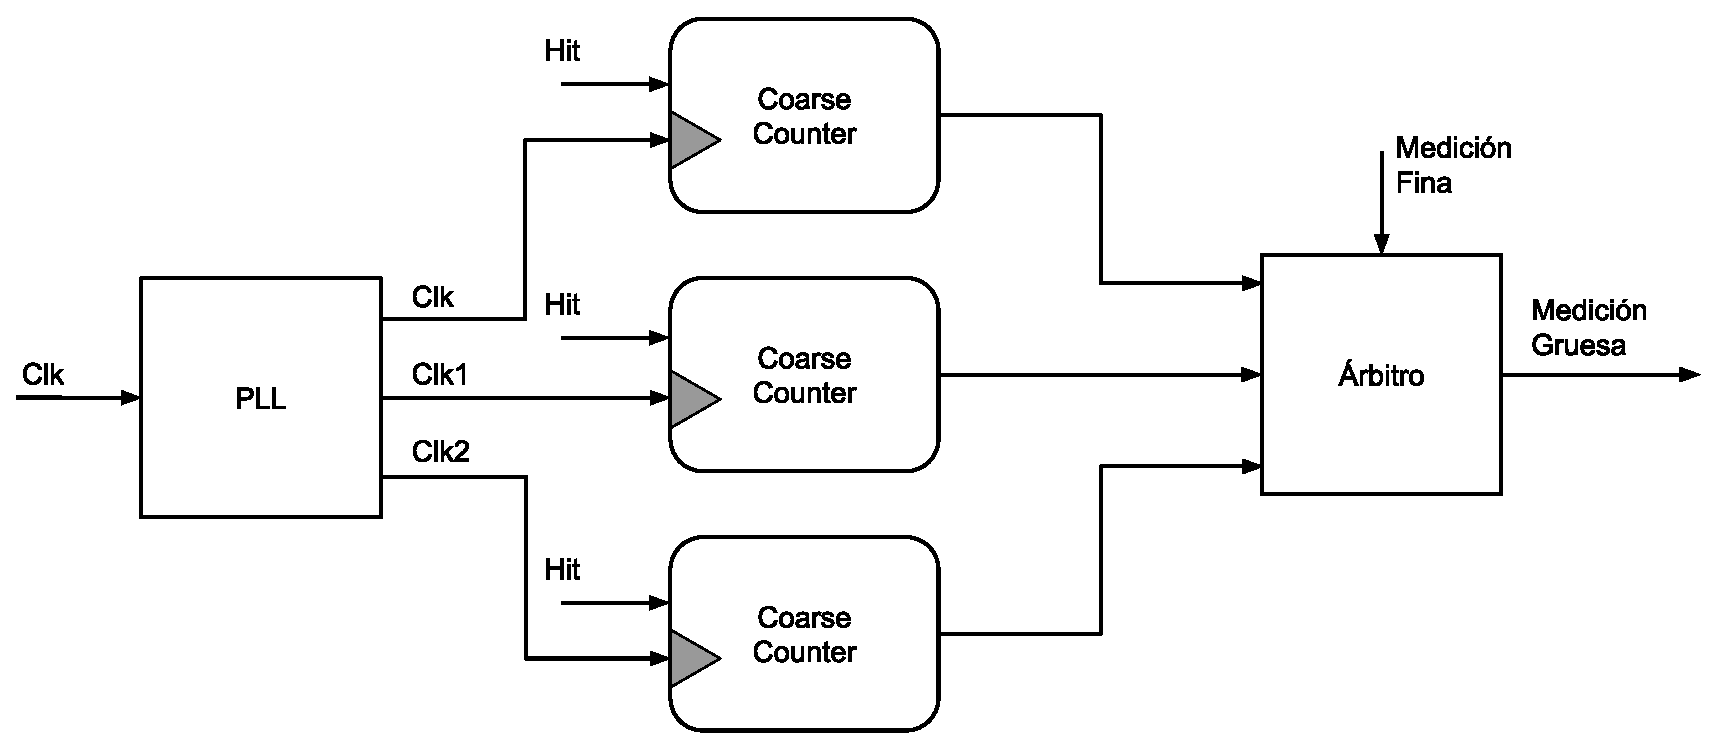
\includegraphics[width=0.75\textwidth]{imagenes/arbiter.eps}
     \caption{Arbitro implementado.}
     \label{fig: arbitro}
\end{figure}

Estos tres relojes inducen cuatro casos a diferenciar, estos se plantearan
para el flanco de entrada pero
puede hacerse de la misma forma para el flanco de salida.\\
El caso base es suponer que el pulso llega antes del flanco de subida de todos los relojes,
como muestra el Caso I de la Figura \ref{fig: casos_arbitro}, o también llegar entre cada par de flancos como muestran los Casos II, III y IV.
Para el primer caso, la línea de retardos captura la señal al inicio de la cadena pues el reloj ocurre cerca de la llegada del pulso, sin embargo
para el resto de casos donde el flanco de reloj ya ocurrió es necesario esperar un período al próximo flanco de reloj, en consecuencia se captura el flanco de entrada
al borde de saturar la cadena de retardos, como muestra la Figura \ref{fig: finos_casos_start}.\\

\begin{figure}[H]
     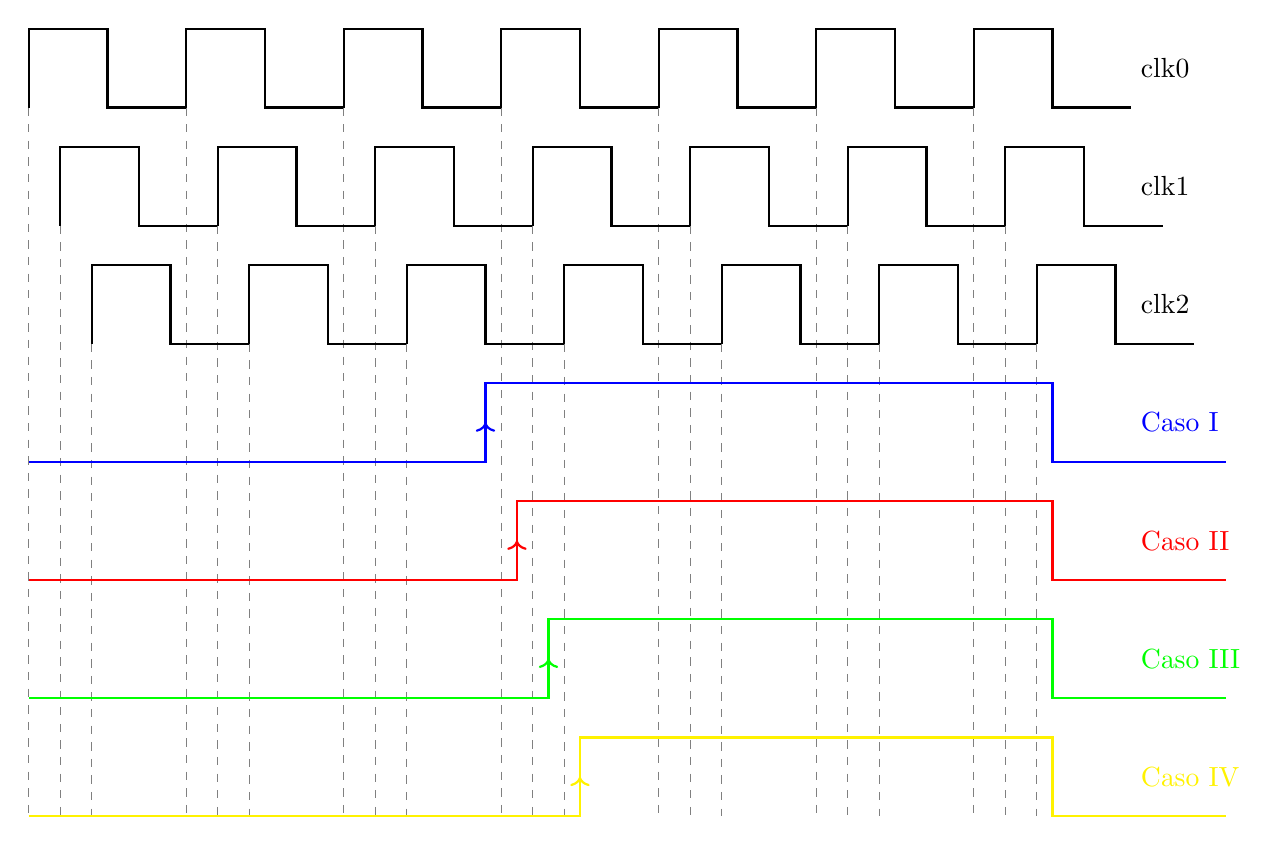
\begin{tikzpicture}
          % Define parameters
          \def\amplitude{1}       % Amplitude of the square waves
          \def\period{2}          % Period of the square waves
          \def\phaseShift{0.2}    % Phase shift for each wave (in terms of period fraction)
          \def\yShift{1.5}        % Vertical shift for each wave
          \def\stepLength{8}      % Total length for the step signal (4 periods)
          \def\stepPhaseShift{0.2}% Phase shift for step signals
      
          \def\Longtotal{15}

          % Draw clk0
          \foreach \x in {0, 2, 4, 6, 8, 10, 12} {
              \draw[thick, black] (\x, 0) -- ++(0, \amplitude) -- ++(1, 0) -- ++(0, -\amplitude) -- ++(1, 0);
              \draw[dashed, gray] (\x, 0) -- (\x, -6*\yShift cm);
          }
          \node[black, right] at (14, 0.5*\amplitude) {clk0};
      
          % Draw clk1
          \foreach \x in {0, 2, 4, 6, 8, 10, 12} {
              \draw[thick, black, yshift=-\yShift cm] (\x + \phaseShift * \period, 0) -- ++(0, \amplitude) -- ++(1, 0) -- ++(0, -\amplitude) -- ++(1, 0);
              \draw[dashed, gray] (\x + \phaseShift * \period, -\yShift cm) -- (\x + \phaseShift * \period, -6*\yShift cm);
          }
          \node[black, right] at (14, 0.5*\amplitude - \yShift) {clk1};
      
          % Draw clk2
          \foreach \x in {0, 2, 4, 6, 8, 10, 12} {
              \draw[thick, black, yshift=-2*\yShift cm] (\x + 2*\phaseShift * \period, 0) -- ++(0, \amplitude) -- ++(1, 0) -- ++(0, -\amplitude) -- ++(1, 0);
              \draw[dashed, gray] (\x + 2*\phaseShift * \period, -2*\yShift cm) -- (\x + 2*\phaseShift * \period, -6*\yShift cm);
          }
          \node[black, right] at (14, 0.5*\amplitude - 2*\yShift) {clk2};
      
          % Draw step signal cases
      
          % Case 1: Rising edge 0.2 to the left of the third clk0 rising edge
          \foreach \x in {6 - 0.2} {
              \draw[thick, blue, yshift=-3*\yShift cm] (0, 0) -- (\x, 0) -- ++(0, \amplitude) -- ++(\stepLength-\period + 1.2, 0) -- ++(0, -\amplitude) -- ++(\Longtotal - \x - \stepLength + \period - 0.6, 0);
              \draw[->, thick, blue] (\x, -3*\yShift cm) -- ++(0, 1/2*\amplitude);
          }
          \node[blue, right] at (14, 0.5*\amplitude - 3*\yShift) {Caso I};
      
          % Case 2: Rising edge 0.2 to the right of the third clk0 rising edge
          \foreach \x in {6 + 0.2} {
              \draw[thick, red, yshift=-4*\yShift cm] (0, 0) -- (\x, 0) -- ++(0, \amplitude) -- ++(\stepLength - \period + 1 - 0.2, 0) -- ++(0, -\amplitude) -- ++(\Longtotal - \x - \stepLength + \period - 1, 0);
              \draw[->, thick, red] (\x, -4*\yShift cm) -- ++(0, 1/2*\amplitude);
          }
          \node[red, right] at (14, 0.5*\amplitude - 4*\yShift) {Caso II};
      
          % Case 3: Rising edge 0.6 to the right of the third clk0 rising edge
          \foreach \x in {6 + 0.6} {
              \draw[thick, green, yshift=-5*\yShift cm] (0, 0) -- (\x, 0) -- ++(0, \amplitude) -- ++(\stepLength - \period +1 -0.6, 0) -- ++(0, -\amplitude) -- ++(\Longtotal - \x - \stepLength + \period - 1.4, 0);
              \draw[->, thick, green] (\x, -5*\yShift cm) -- ++(0, \amplitude/2);
          }
          \node[green, right] at (14, 0.5*\amplitude - 5*\yShift) {Caso III};
      
          % Case 4: Rising edge 1 to the right of the third clk0 rising edge
          \foreach \x in {6 + 1} {
              \draw[thick, yellow, yshift=-6*\yShift cm] (0, 0) -- (\x, 0) -- ++(0, \amplitude) -- ++(\stepLength - \period +1 -1, 0) -- ++(0, -\amplitude) -- ++(\Longtotal - \x - \stepLength + \period - 1.8, 0);
              \draw[->, thick, yellow] (\x, -6*\yShift cm) -- ++(0, \amplitude/2);
          }
          \node[yellow, right] at (14, 0.5*\amplitude - 6*\yShift) {Caso IV};
     \end{tikzpicture}
     \caption{Todos los casos posibles de arbitraje para el flanco Start}
     \label{fig: casos_arbitro}
\end{figure}

\begin{figure}[H]
     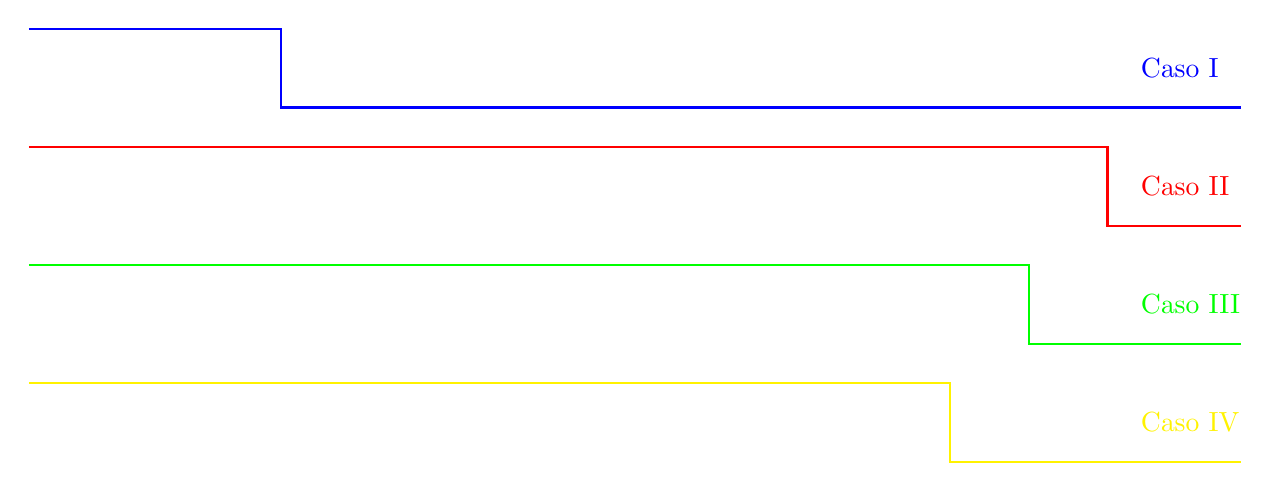
\begin{tikzpicture}
          % Define parameters
          \def\amplitude{1}       % Amplitude of the square waves
          \def\period{2}          % Period of the square waves
          \def\phaseShift{0.2}    % Phase shift for each wave (in terms of period fraction)
          \def\yShift{1.5}        % Vertical shift for each wave
          \def\stepLength{8}      % Total length for the step signal (4 periods)
          \def\stepPhaseShift{0.2}% Phase shift for step signals
      
          \def\Longtotal{15}
          
          %%Casos en cade fina:
          % Case 1: Rising edge 0.2 to the left of the third clk0 rising edge
          \foreach \x in {3 + 0.2} {
              \draw[thick, blue] (0, \amplitude) -- (\x, \amplitude) -- ++(0, -\amplitude) -- ++(\Longtotal - \x , 0);
          }
          \node[blue, right] at (14, 0.5*\amplitude) {Caso I};

           % Case 2: Rising edge 0.2 to the right of the third clk0 rising edge
           \foreach \x in {13.5 + 0.2} {
               \draw[thick, red, yshift=-\yShift cm] (0, \amplitude) -- (\x, \amplitude) -- ++(0, -\amplitude) -- ++(\Longtotal - \x , 0);
           }
           \node[red, right] at (14, 0.5*\amplitude - \yShift) {Caso II};

           % Case 3: Rising edge 0.2 to the right of the third clk0 rising edge
           \foreach \x in {12.5 + 0.2} {
               \draw[thick, green, yshift=-2*\yShift cm] (0, \amplitude) -- (\x, \amplitude) -- ++(0, -\amplitude) -- ++(\Longtotal - \x , 0);
           }
           \node[green, right] at (14, 0.5*\amplitude - 2*\yShift) {Caso III};

           % Case 4: Rising edge 0.2 to the right of the third clk0 rising edge
           \foreach \x in {11.5 + 0.2} {
               \draw[thick, yellow, yshift=-3*\yShift cm] (0, \amplitude) -- (\x, \amplitude) -- ++(0, -\amplitude) -- ++(\Longtotal - \x , 0);
           }
           \node[yellow, right] at (14, 0.5*\amplitude - 3*\yShift) {Caso IV};

     \end{tikzpicture}
      \caption{Registro \textit{Start} de la cadena de retardos para cada caso de arbitraje.}
      \label{fig: finos_casos_start}
\end{figure}

Si analizamos cada caso con su contador grueso entonces obtendríamos los resultados que se presentan en la Tabla \ref{tabla: arbitro}.
Rápidamente nos podemos dar cuenta que si todos los contadores gruesos tienen la misma respuesta entonces el resultado de cualquiera de ellos es correcto,
pero si no son iguales y el pulso es detectado en el extremo de la cadena, sabemos con certeza que la cuenta correcta es de tres períodos,
pues el período incompleto está codificado en la respuesta fina. Es entonces posible conociendo las cuatro posibles condiciones de cuentas gruesas generar 
una respuesta apoyada en cuatro referencias: tres contadores y la respuesta fina.

\begin{table}[H]
     \centering
     \begin{tabular}{|l|c|c|c|}
     \hline
     Coarse counter según: & clk0 & clk1 & clk2 \\ \hline
     Caso I                & 4    & 4    & 4    \\ \hline
     Caso II               & 3    & 4    & 4    \\ \hline
     Caso III              & 3    & 3    & 4    \\ \hline
     Caso IV               & 3    & 3    & 3    \\ \hline
     \end{tabular}
     \caption{Cuenta gruesa del ejemplo presentado en la Figura \ref{fig: casos_arbitro}, según cada reloj generado por el PLL.}
     \label{tabla: arbitro}
\end{table}


\subsection{Implementación}
Finalmente se implementó la arquitectura presentada en \cite{machado_novel_2018} que se repite en la Figura \ref{fig: TDC}.
\begin{figure}[H]
     \centering
     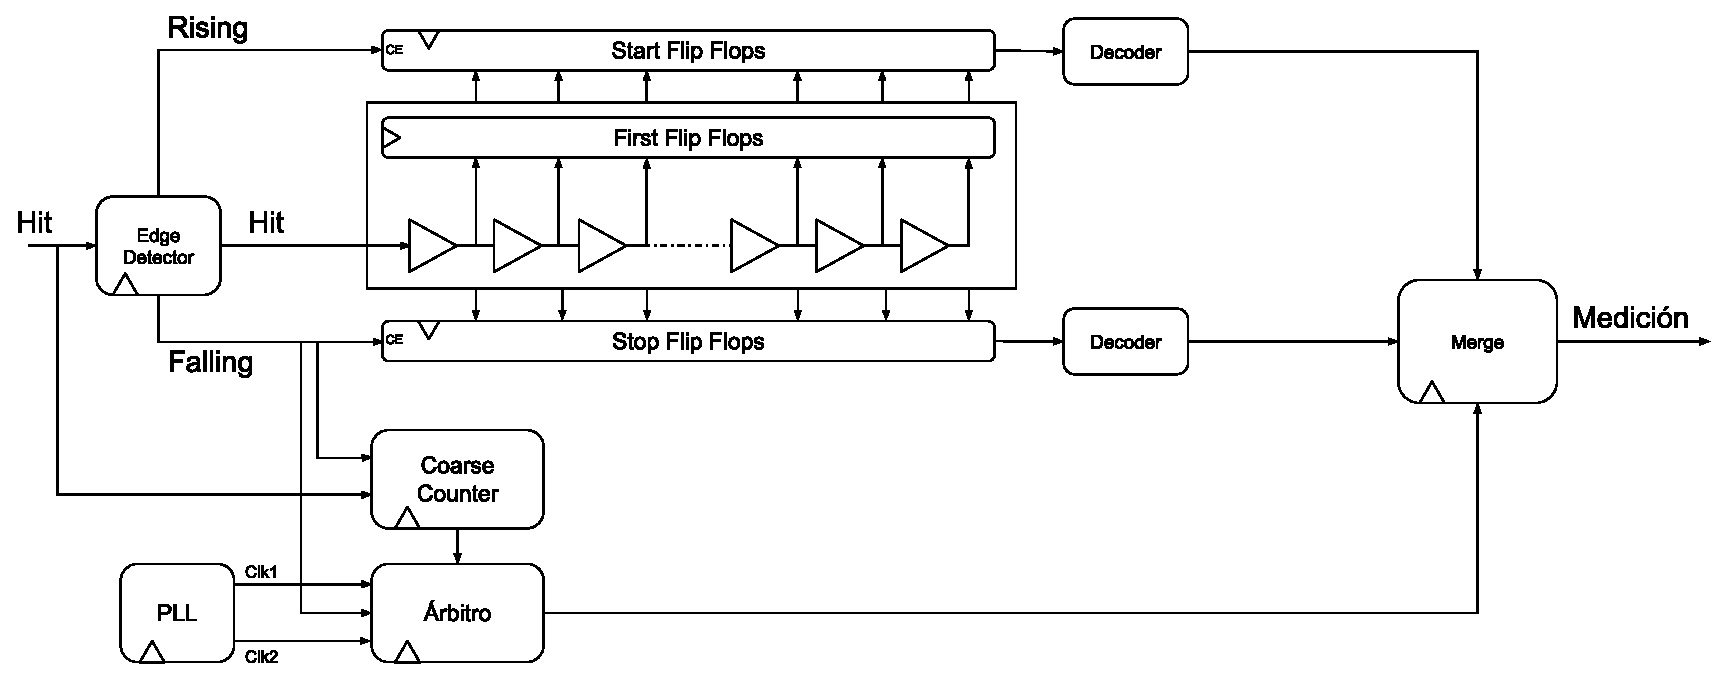
\includegraphics[width=0.9\textwidth]{imagenes/arq_tdc.eps}
     \caption{Arquitectura del TDC. Se ignora el ruteo del clock.}
     \label{fig: TDC}
\end{figure}

Además para poder medir y procesar los datos se realizó el esquema de la Figura \ref{fig: esquema}.
\begin{figure}[H]
      \centering
      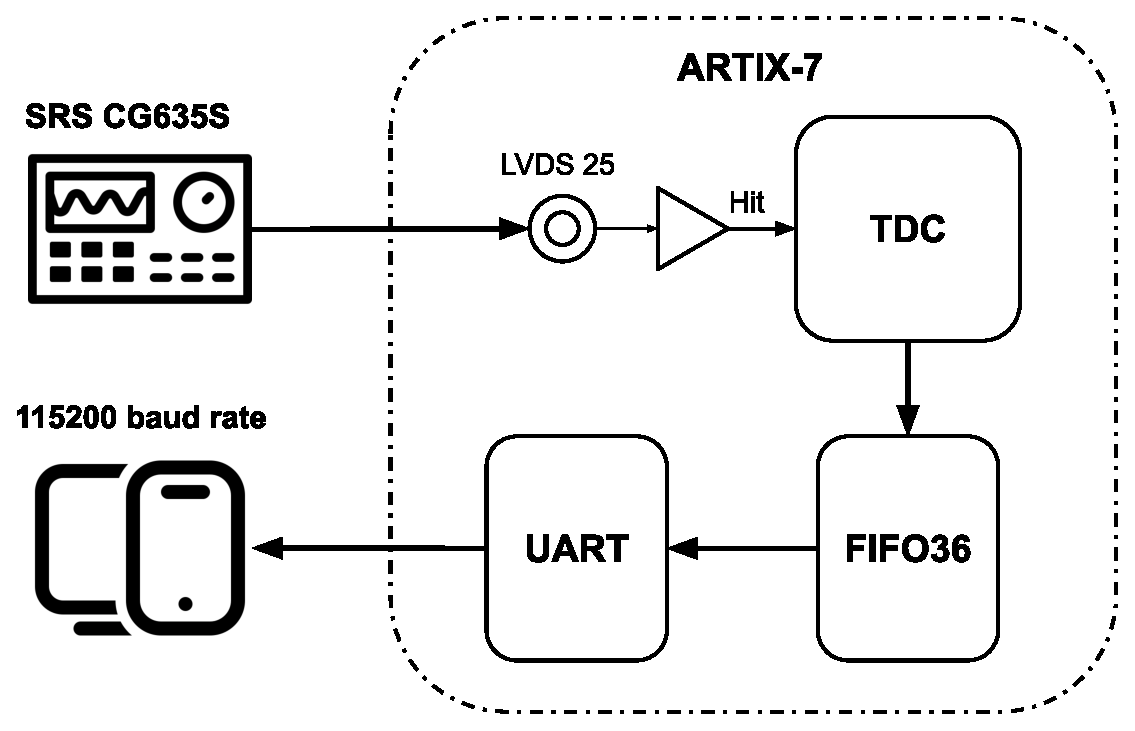
\includegraphics[width=0.4\textwidth]{imagenes/TDC-functional-blocks.eps}
      \caption{Esquema de medición}
      \label{fig: esquema}
\end{figure}
El generador de señales ingresa en diferencial a los conectores SMA de los puertos \textit{GPIO} J33 y J34, de la
placa de desarrollo AC701, que contiene una FPGA Xilinx Artix-7. Esta implementa el TDC que al ser activado
realiza consecutivamente mediciones hasta llenar una memoria FIFO de 32 bits de largo, y 1024 palabras de profundidad.
A su vez, cuando el usuario decide obtener los datos, se desactiva el TDC y la FPGA se conecta por puerte serie 
para descargar la información, para lo cual se ha confeccionado un script en \textit{python} que recibe los datos,
separa cada palabra de 32 bits en sus 10 bits de stop, 10 bits de start, y 12 bits de contador grueso, los
transforma en el valor decimal correspondiente y los guarda en un archivo \textit{``.txt''}. Luego otro script se encarga
de graficar una rápida visualización de los resultados. Tanto la conexión serie y la escritura/lectura de la memoria fueron
probados en distintos casos para descartar errores.\\

El código, como algunos recursos de lectura utilizados, y detalles de implementación generales fueron publicados en el
siguiente \href{https://github.com/Miquefil/TDC-in-Artix-7}{repositorio de Github}.


\clearpage
\section{Resultados}
Haciendo uso de un generador de reloj ``SRS CG635S'' se realizó la prueba de densidad de código
con una frecuencia de $5.123456$ MHz, obteniendo histogramas los
distribuidos para el flanco de start y de stop que se muestran en la Figura \ref{fig: histogramas_magic}.
\begin{figure}[H]
     \centering
     \begin{subfigure}{0.45\textwidth}
           \centering
           \resizebox{\linewidth}{!}{
           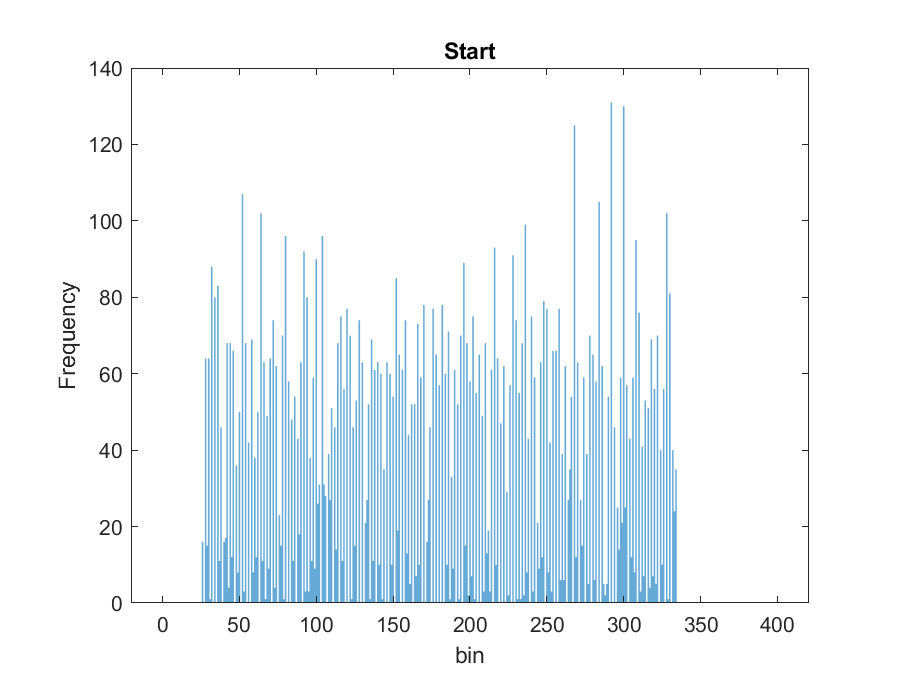
\includegraphics[]{imagenes/histograma_start.eps}
           }
     \end{subfigure}%
     \hspace{10pt}%
     \begin{subfigure}{0.45\textwidth}
           \centering
           \resizebox{\linewidth}{!}{
           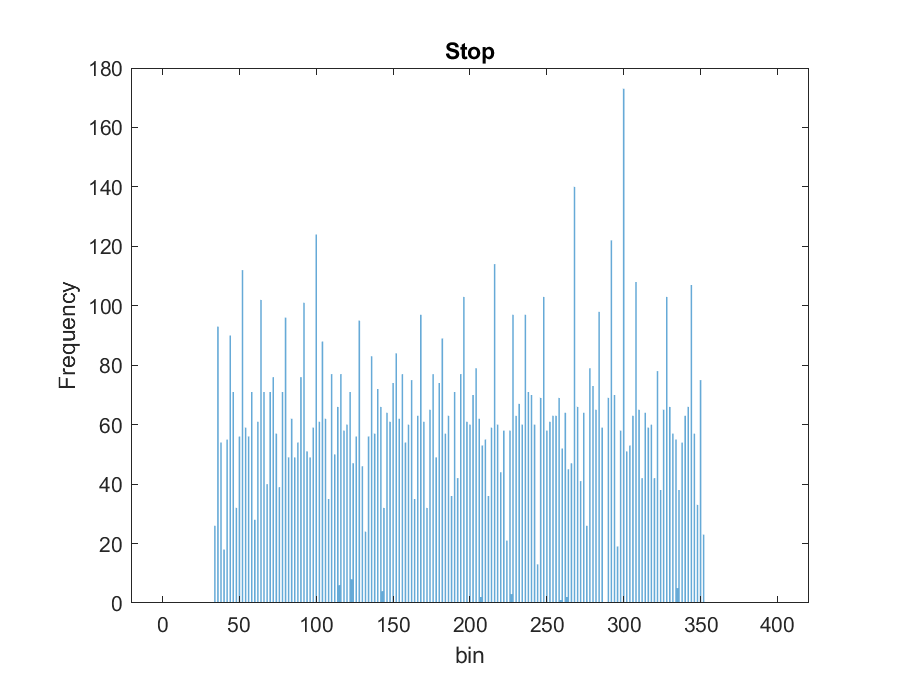
\includegraphics[]{imagenes/histograma_stop.eps}
           }
     \end{subfigure}
     \caption{Histogramas del flanco de subida y flanco de bajada, para 10240 mediciones
     utilizando una frecuencia de $5.123456$MHz .}
     \label{fig: histogramas_magic}
\end{figure}%

Es posible ver que los flancos de subida y bajada no se propagan de igual forma, pues no se presenta
la misma cantidad de bines para cada histograma. Podemos decir que el flanco stop se propaga de forma más
rápida que el flanco start, pues alcanza un número de retardos mayor, 
lo que quiere decir que las celdas de retardo son más cortas cuando propagan una transición ``1-0''.
Además, prestando especial atención al histograma stop se puede observar que los bines pares no son alcanzados,
lo que sugiere que una única celda de retardo es demasiado pequeña para la velocidad de propagación del flanco.\\

% Esto es completamente posible, ya que puede ocurrir que al implementar una compuerta los transistores complementarios
% no sean exactamente iguales. Tomemos como ejemplo la compuerta inversora \ref{fig: buffer_inversor}. Cuando la entrada está
% en alto, el N-MOS entra en juego colocando un estado bajo a la salida. A la inversa, entra en juego el transistor PMOS. Esto
% pone en evidencia que si las características dinámicas de ambos transistores no son iguales, entonces la propagación de una transición
% alto-bajo/bajo-alto se dará de forma distinta.
% \begin{figure}[H]
%       \centering
%       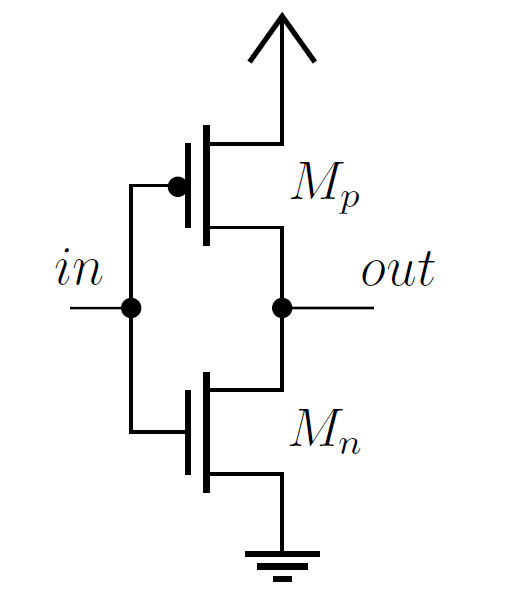
\includegraphics[width=0.35\textwidth]{imagenes/buffer_inversor.png}
%       \caption{Circuito del buffer inversor.}
%       \label{fig: buffer_inversor}
% \end{figure}

\begin{figure}[h]
     \centering
     \begin{minipage}{0.5\textwidth}
          Esto es completamente posible, ya que puede ocurrir que al implementar una compuerta los transistores complementarios
           no sean exactamente iguales. Tomemos como ejemplo la compuerta inversora \ref{fig: buffer_inversor}. Cuando la entrada está
           en alto, el NMOS entra en juego colocando un estado bajo a la salida. A la inversa, entra en juego el transistor PMOS. Esto
           pone en evidencia que si las características dinámicas de ambos transistores no son iguales, entonces la propagación de una transición
           alto-bajo/bajo-alto se dará de forma distinta.
      \end{minipage}%
     \begin{minipage}{0.5\textwidth}
         \centering
         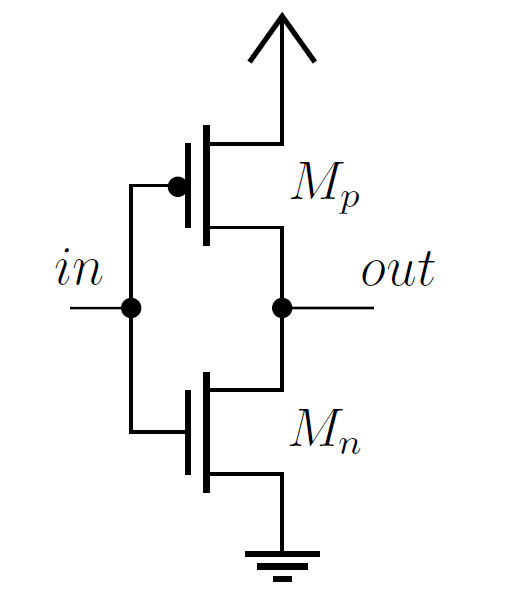
\includegraphics[width=0.4\linewidth]{imagenes/buffer_inversor.png}
         \caption{Circuito del buffer inversor.}
         \label{fig: buffer_inversor}
     \end{minipage}     
 \end{figure}

Luego, para el flanco stop se utiliza desde el bin número $35$, hasta el bin número $353$, lo que nos
da una cantidad de bines utilizados $N_c^{\text{stop}} = 318$, mientras que el flanco start
ocupa desde el bin número $27$, hasta el bin $335$, utilizando un total de $N_c^{\text{start}} = 308$
elementos de retardo. Con esto se puede calcular que el retardo de cada celda es:
\begin{align}
     \hat{\tau}_{\text{stop}} = 15.72 \text{ ps} \; , && \hat{\tau}_{\text{start}} = 16.23 \text{ ps}
\end{align}
Con esto se pueden construir los histogramas de linealidad, tal como muestran las Figuras \ref{fig: linealidad_stop}, \ref{fig: linealidad_start}, 
utilizando las ecuaciones \ref{eq: tau_medio}, \ref{eq: DNL}, \ref{eq: INL}.

\begin{figure}[H]
      \centering
      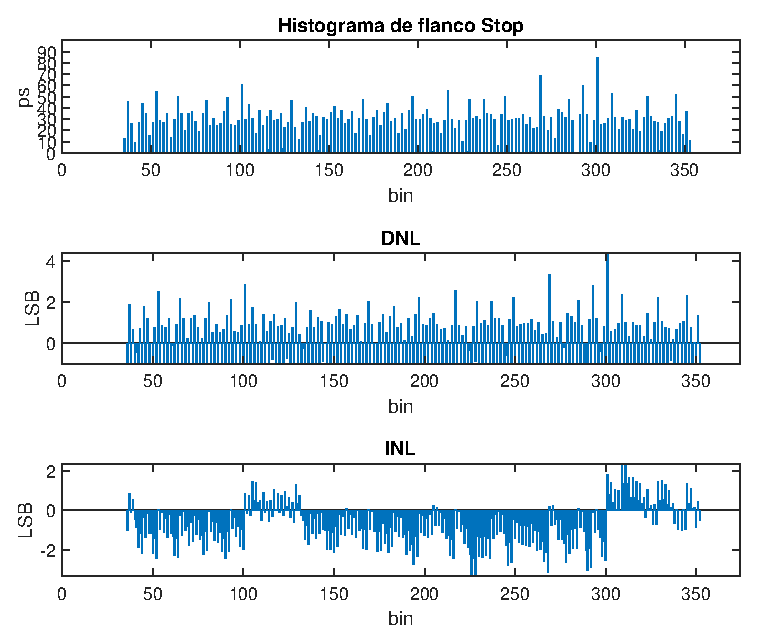
\includegraphics[width=0.75\textwidth]{imagenes/linealidad_stop.eps}
      \caption{Histogramas de linealidad obtenidos en la prueba de densidad de código para el flanco de stop.}
      \label{fig: linealidad_stop}
\end{figure}

\begin{figure}[H]
      \centering
      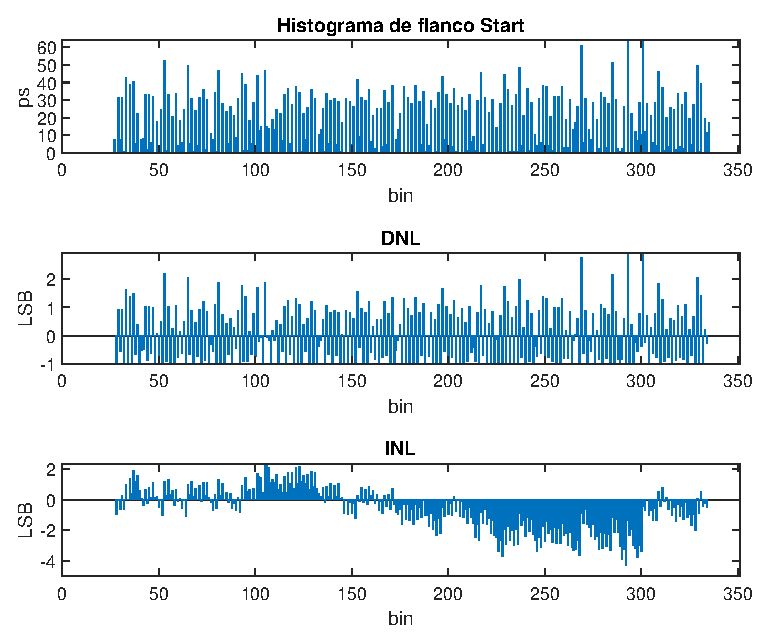
\includegraphics[width=0.75\textwidth]{imagenes/linealidad_start.eps}
      \caption{Histogramas de linealidad obtenidos en la prueba de densidad de código para el flanco de start.}
      \label{fig: linealidad_start}
\end{figure}

\clearpage

Se procedió a realizar un experimento de 10240 mediciones para seis frecuencias distintas.
Para cada experimento, el tiempo fino es calculado tal como muestra el esquema de la Figura \ref{fig: arqui_tdl}, y lleva a:
\begin{equation}
     t_\text{fino} = n_\text{start} \; \hat{\tau_\text{start}} - n_\text{stop} \; \hat{\tau_\text{stop}} \; .
     \label{eq: t_fino}
\end{equation}
\begin{figure}[H]
     \centering
     \begin{subfigure}[t]{0.45\textwidth} % [t] aligns the top of the subfigure
           \centering
           \resizebox{\linewidth}{!}{
               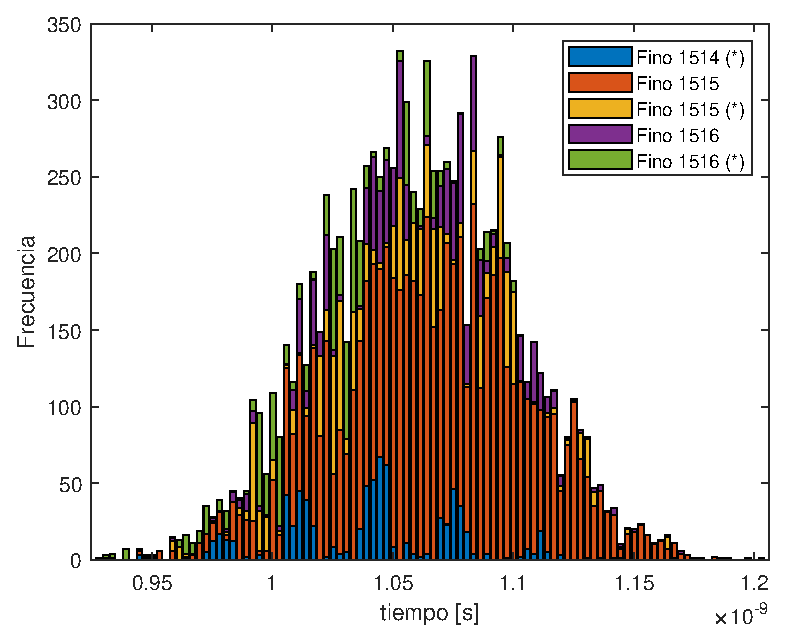
\includegraphics[width=0.75\textwidth]{imagenes/histograma_66k.eps}
           }
           \caption{Histograma de mediciones finas.}
           \label{fig: histograma_66}
     \end{subfigure}%
     \hspace{10pt}%
     \begin{subfigure}[t]{0.45\textwidth} % [t] aligns the top of the subfigure
           \centering
           \resizebox{\linewidth}{!}{
               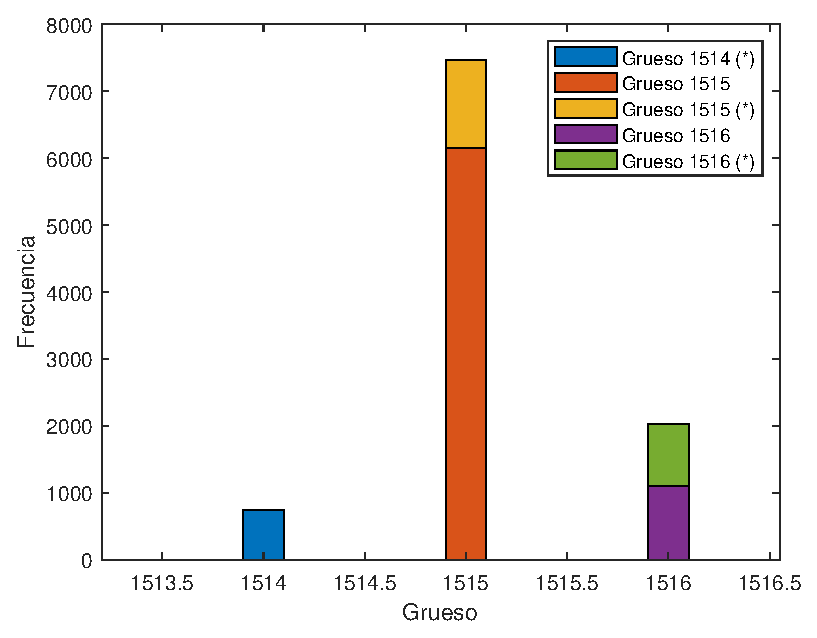
\includegraphics[]{imagenes/histograma_coarse_66k.eps}
           }
           \caption{Histograma de mediciones gruesas.}
     \end{subfigure}
     \caption{Histograma de 10240 mediciones utilizando una frecuencia de $f=66$ kHz, $t_{\text{on}}=7.57 \; \mu$s. 
     Se indican con un asterisco aquellas mediciones cuyo contador grueso debió ser corregido.}
\end{figure}

\begin{figure}[H]
     \centering
     \begin{subfigure}[t]{0.45\textwidth} % [t] aligns the top of the subfigure
           \centering
           \resizebox{\linewidth}{!}{
               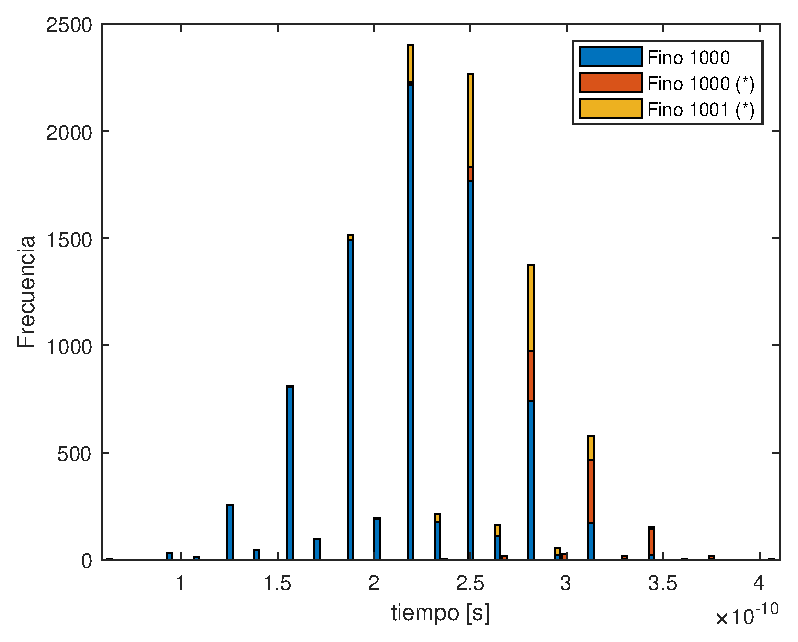
\includegraphics[width=0.75\textwidth]{imagenes/histograma_100k.eps}
           }
           \caption{Histograma de mediciones finas.}
           \label{fig: histograma_66}
     \end{subfigure}%
     \hspace{10pt}%
     \begin{subfigure}[t]{0.45\textwidth} % [t] aligns the top of the subfigure
           \centering
           \resizebox{\linewidth}{!}{
               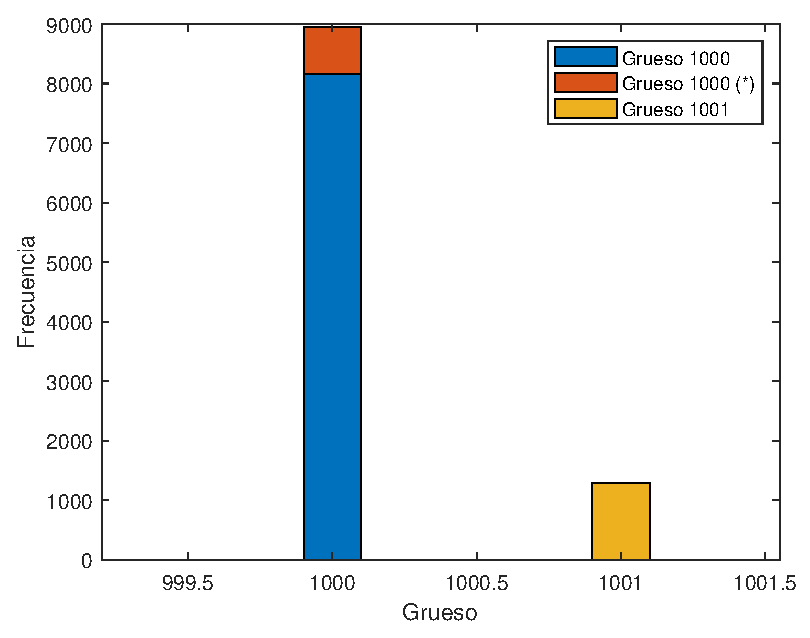
\includegraphics[]{imagenes/histograma_coarse_100k.eps}
           }
           \caption{Histograma de mediciones gruesas.}
     \end{subfigure}
     \caption{Histograma de 10240 mediciones utilizando una frecuencia de $f=100$ kHz, $t_{\text{on}}=5 \; \mu$s. 
     Se indican con un asterisco aquellas mediciones cuyo contador grueso debió ser corregido.}
\end{figure}

\clearpage

\begin{figure}[H]
     \centering
     \begin{subfigure}[t]{0.45\textwidth} % [t] aligns the top of the subfigure
           \centering
           \resizebox{\linewidth}{!}{
               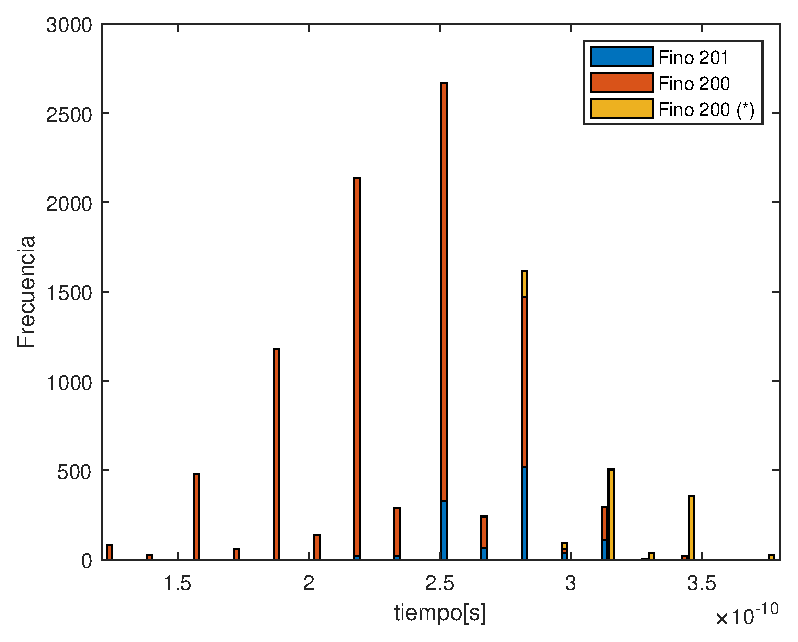
\includegraphics[width=0.75\textwidth]{imagenes/histograma_500k.eps}
           }
           \caption{Histograma de mediciones finas.}
           \label{fig: histograma_500}
     \end{subfigure}%
     \hspace{10pt}%
     \begin{subfigure}[t]{0.45\textwidth} % [t] aligns the top of the subfigure
           \centering
           \resizebox{\linewidth}{!}{
               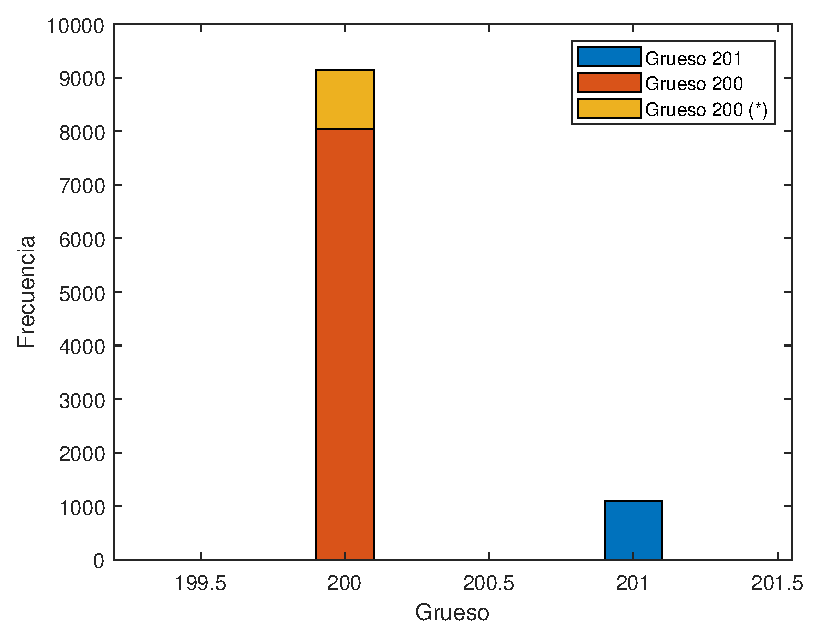
\includegraphics[]{imagenes/histograma_coarse_500k.eps}
           }
           \caption{Histograma de mediciones gruesas.}
     \end{subfigure}
     \caption{Histograma de 10240 mediciones utilizando una frecuencia de $f=500$ kHz, $t_{\text{on}}=1 \; \mu$s. 
     Se indican con un asterisco aquellas mediciones cuyo contador grueso debió ser corregido.}
\end{figure}


En resumen, se obtuvieron los resultados que muestra la Tabla \ref{tabla: res_med_1}. Para presentar los datos, se
transportaron las mediciones finas a su concentración positiva. Por ejemplo, si se debe medir un ancho de pulso
de $45.45$ relojes, entonces podríamos obtener dos resultados correctos: $45$ relojes de medición gruesa y $0.45 \; T$
de medición fina, o $46$ relojes de medición gruesa y $-0.55 \; T$ de medición fina. Como el árbitro no fue
implementado, un gran porcentaje de las muestras contienen errores de sincronización, y estas son indicadas
con un asterisco. En la Figura \ref{fig: histograma_500} se observa que gran parte de las mediciones
se realizan con una cantidad gruesa de $200$ relojes, cuyo período es de $5$ ns, conteniendo toda 
la información necesaria ($200 \cdot T = 1 \; \mu$s), entonces la medición fina es un sesgo. Para el caso en que se mide
$201$ períodos de reloj, la medición fina es una campana concentrada en $-4.68$ ns, pero que para la facilidad del lector
se representa en su forma complementaria positiva al sumarle un período.

\begin{table}[!htpb]
     \centering
     \begin{tabular}{cccc}
     \hline
     Frecuencia         & $E[X]$   & $ \sigma[X]$ & Error $[$ps$]$ \\ \hline
     66 kHz             & 1.06 ns  & 39.6 ps      & 303            \\ \hline
     100 kHz            & 323 ps   & 35 ps        & 323            \\ \hline
     500 kHz            & 338 ps   & 27.1 ps      & 338            \\ \hline
     1.225 MHz          & 3.43 ns  & 29.8 ps      & 269            \\ \hline
     2 MHz              & 271 ps   & 23.9 ps      & 271            \\ \hline
     3.3 MHz            & 1.78 ns  & 26.7 ps      & 272            \\ \hline
     5 MHz              & 286 ps   & 25.1 ps      & 286            \\ \hline
     \end{tabular}
     \caption{Parámetros de tiempo fino extraídos de cada experimento, cada uno con 10240 mediciones.
     Se indica como $E[X]$ a la media, y $\sigma[X]$ a la desviación estándar.}
     \label{tabla: res_med_1}
\end{table}


Se calculó el error estimado como $E[X] - t_\text{on}$, donde $t_\text{on}$ es el semiperíodo de la frecuencia
ingresada en el generador de señales, y $E[X]$ la media de las mediciones finas sincronizadas.
Queda en evidencia que existe un sesgo para todos los experimentos de alrededor de $300$ ps. Aunque es difícil explicar este
hecho, la primer conjetura es que este provenga del tiempo de crecimiento/caída del generador,
sin embargo este es $\leq 80$ps para todo el rango de frecuencias, que se pudo constatar mediante un osciloscopio.
No obstante es importante tener en cuenta la no linealidad de la cadena, que en particular afecta
la forma de calcular el tiempo fino en la Ecuación \ref{eq: t_fino}. Como no se utiliza el mismo tiempo de retardo ($\tau$) medio
para la propagación de subida y de bajada, entonces existe un error acumulado a medida que los flancos avanzan dentro
de la cadena. Para verificar esto, a continuación se grafica un histograma de dos dimensiones para cada experimento, esto es:
para cada valor $n_\text{start}$ del eje $x$ se grafica el histograma de diferencia $n_\text{start}-n_\text{stop}$ en el eje $y$  ,
en otras palabras se grafica la diferencia de bines en función de dónde se encontró el bin start. Esto nos permite independizarnos
de la temporalidad de los experimentos realizados, y observar el comportamiento de los retardos en función de la posición
dentro de la cadena. 

\begin{figure}[H]
     \centering
     \begin{minipage}{0.45\textwidth}
         \centering
         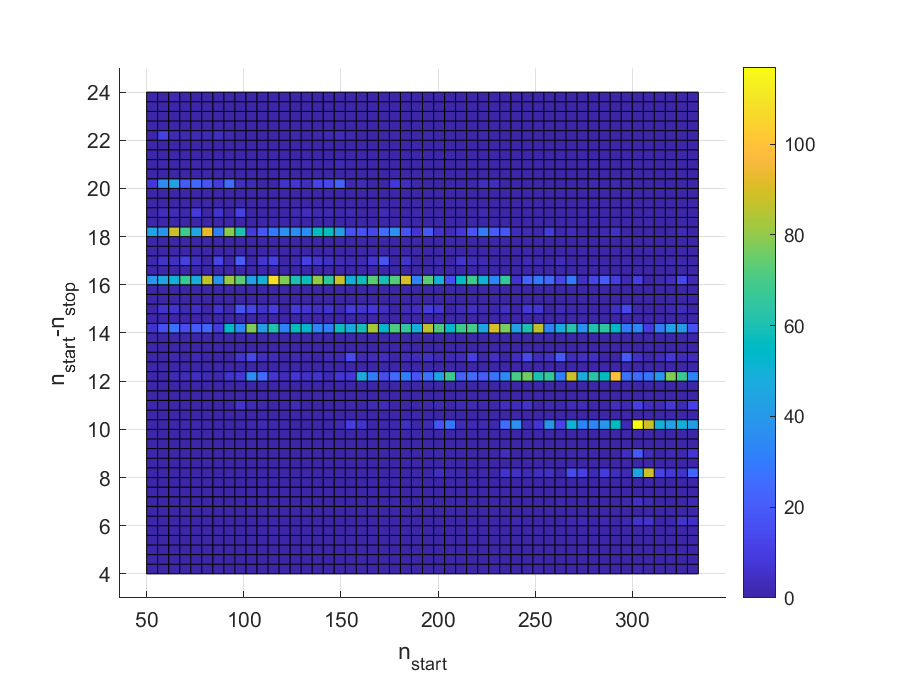
\includegraphics[width=\textwidth]{imagenes/start-stop_100k.eps} % Replace with your figure path
         \caption{$f = 100$ kHz}
     \end{minipage}\hfill
     \begin{minipage}{0.45\textwidth}
         \centering
         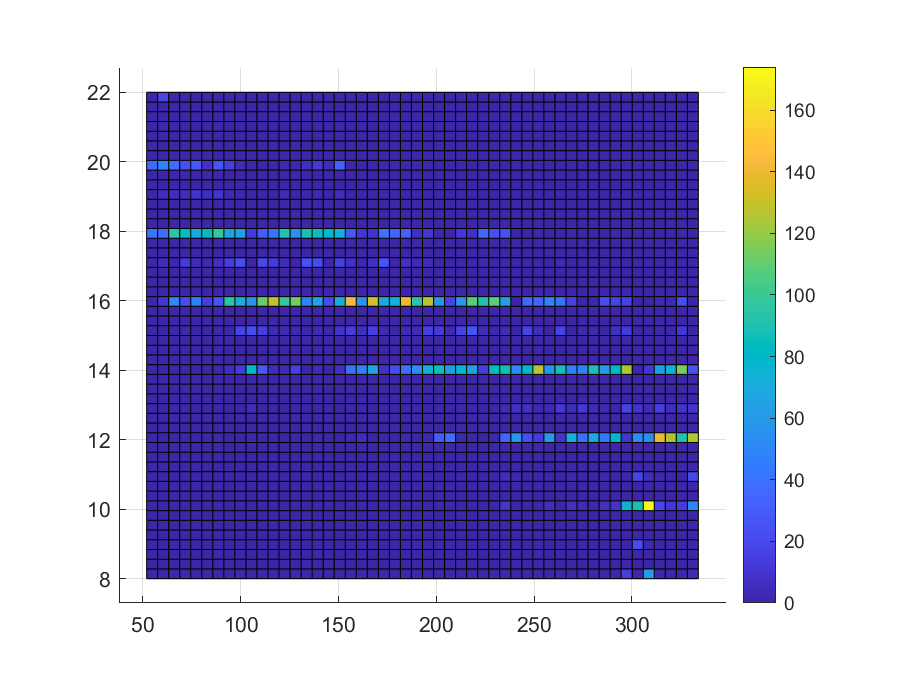
\includegraphics[width=\textwidth]{imagenes/start-stop_500k.eps} % Replace with your figure path
         \caption{$f = 500$ kHz}
     \end{minipage}
     
     \vspace{0.5cm} % Space between rows
     
     \begin{minipage}{0.45\textwidth}
         \centering
         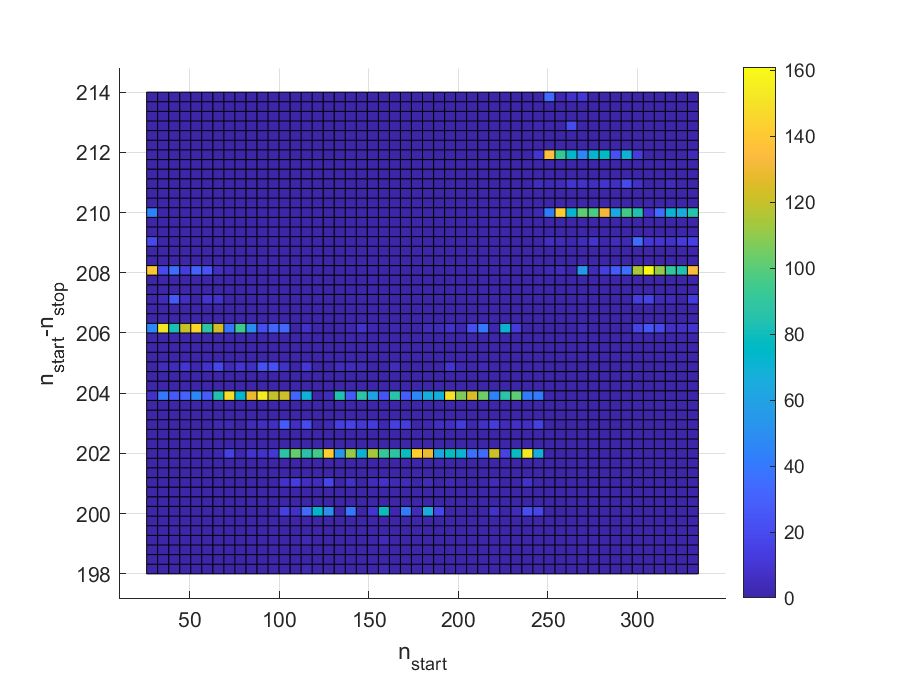
\includegraphics[width=\textwidth]{imagenes/start-stop_1225M.eps} % Replace with your figure path
         \caption{$f = 1.225$ MHz}
     \end{minipage}\hfill
     \begin{minipage}{0.45\textwidth}
         \centering
         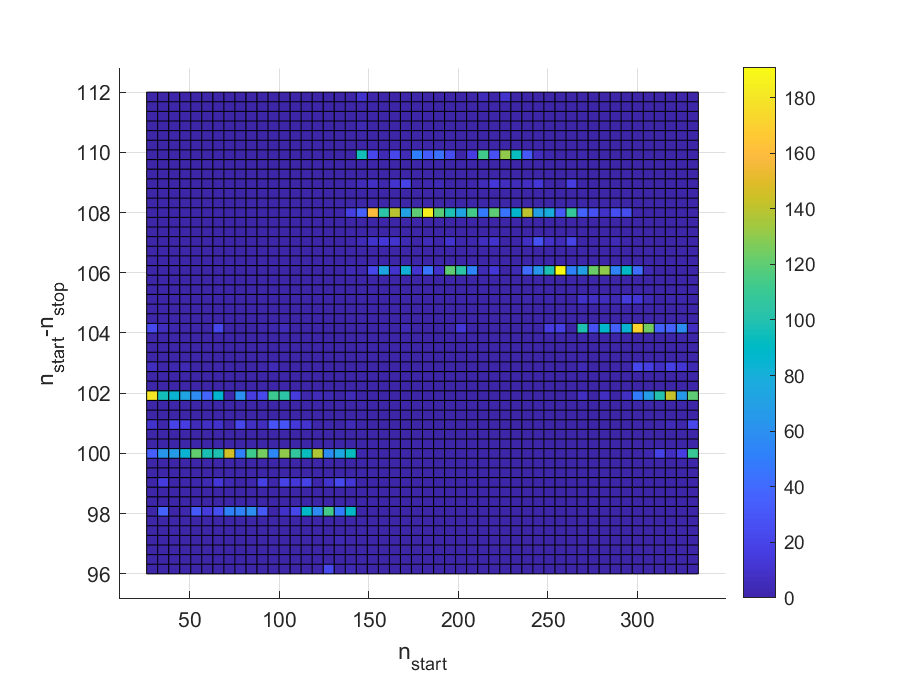
\includegraphics[width=\textwidth]{imagenes/start-stop_3M3.eps} % Replace with your figure path
         \caption{$f = 3.3$ MHz}
     \end{minipage}
     \caption{Histograma que muestra la diferencia elementos de retardo start-stop en función
          de dónde se detectó el flanco de start dentro de la cadena, para cada experimento.}
\end{figure}

De estos resultados se realizaron dos conjeturas:
 \begin{itemize}
     \item Cuando la frecuencia es múltiplo de la frecuencia de reloj ($500$ kHz, $100$ kHz, $2$ MHz, $5$ MHz),
     se puede observar que la diferencias tienden a cero cuando se avanza en la cadena. Es posible entonces pensar que las no linealidades
     acumuladas a medida que se avanza en la cadena tienden a compensarse, de forma que la diferencia tiende a cero,
     tal como se espera de una frecuencia exacta donde el contador grueso contiene toda la información necesaria.
     \item Cuando la frecuencia no es múltiplo del reloj, y por lo tanto el tiempo fino a medir es distinto de cero,
     se pueden observar distintos patrones de dispersión. Si tomamos la tendencia de este histograma, se puede observar
     que la dispersión pico a pico es de al rededor de $10$ bines. El corte que se observa ocurre principalmente porque 
     dependiendo de la cantidad de tiempo fino que se debe medir, a medida que el pulso avanza en fase dentro
     de la cadena, $n_\text{stop}$ y $n_\text{start}$ también avanzan en fase y por lo tanto se van transfieriendo cantidad de bines.
     Es decir, si tuvieramos una cadea de $300$ elementos y el tiempo fino total a medir es de $200$ bines, en un primer momento podemos encontrar que $n_\text{start} = 80$
     y $n_\text{stop} = 280$, pero si siguen avanzando en fase podemos llegar a encontrar $n_\text{start} = 200$ y $n_\text{stop} = 100$ (\ref{fig: no linealidades}).
     Cuando existe un cruce de este tipo, las no linealidades acumuladas en los extremos opuestos de la cadena son tan distintos que
     producen un salto en el histograma.
 \end{itemize}

 \begin{figure}[H]
     \centering
     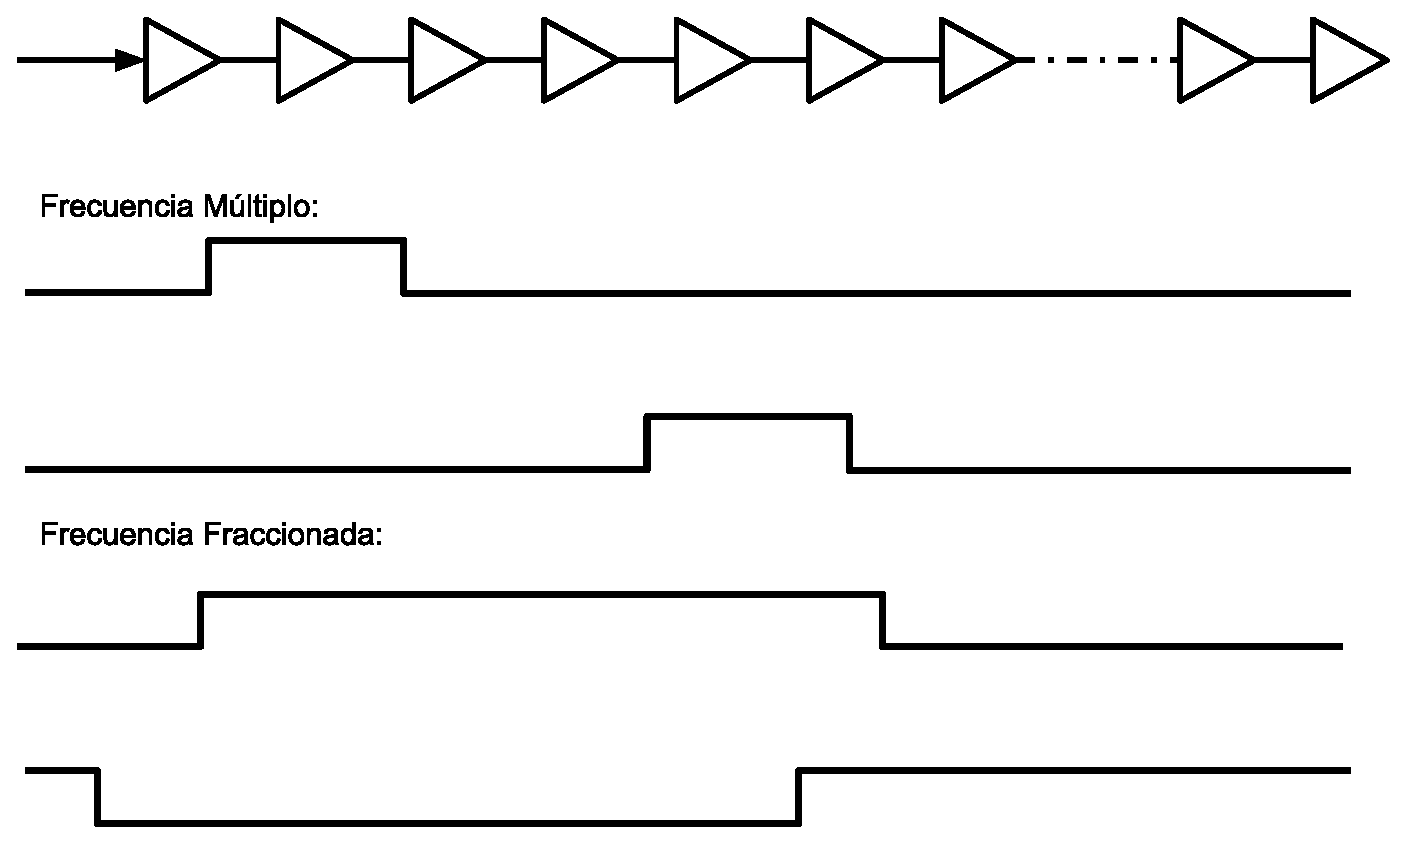
\includegraphics[width=0.75\textwidth]{imagenes/no-linealidades.eps}
     \caption{Explicación de la no linealidad observada en los histogramas.}
     \label{fig: no linealidades}
 \end{figure}


 \subsection{Calibración}
 Para mejorar la performance del TDC, se procedió a realizar cambios de implementación en el diseño final. Originalmente 
 la ubicación y cableado realizado con la ayuda de la herramienta se presenta en la Figura \ref{fig: floorplan_0}. 
 En principio se acortó la cadena y se la colocó a partir del slice $Y111$. Con la ayuda del
 parámetro de colocación fija \texttt{(* LOC = ``SLICE\_X84Y111'' *)} en el primer \textit{Carry4}, a continuación del buffer 
 de reloj como indica \cite{machado_novel_2018}, la herramienta comprende que el el resto de elementos deben ser colocados en línea. 
 Luego para que el ruteo desde 
 los retardos hasta sus registros sean lo más uniformes posibles, se generó la instanciación de cada uno de estos mediante un script en
 \textit{python}, lo que permitió crear la columna de flip flops de start y stop a continuación de estos, como muestra la Figura \ref{fig: floorplan_retardos}.
 Además utilizando restricciones (constraints en el software \textit{Vivado}) se logró excluir cualquier otro elemento dentro de la región donde se instanció la cadena de retardos,
 de forma tal que las conexiones no se vean intervenidas, obteniendo un ruteo uniforme como muestra la Figura \ref{fig: ruteo}. 
 Para lograrlo se muestran los \textit{P\_blocks} en la Figura \ref{fig: floorplan_pblocks}, donde cada
 rectángulo pertenece a un constraint distinto. En el \textit{Pblock\_fine} se colocaron
 únicamente la cadena de retardos y sus respectivos registros, y el \textit{Pblock\_decode} sólo permite la colocación de compuertas que 
 pertenezcan a los bloques de decodificación. Es así que los ruteos desde \textit{Pblock\_fine} hacia \textit{Pblock\_decode} son lo más
 uniforme posibles sin recurrir a un ruteo manual.

 \begin{figure}[H]
      \centering
      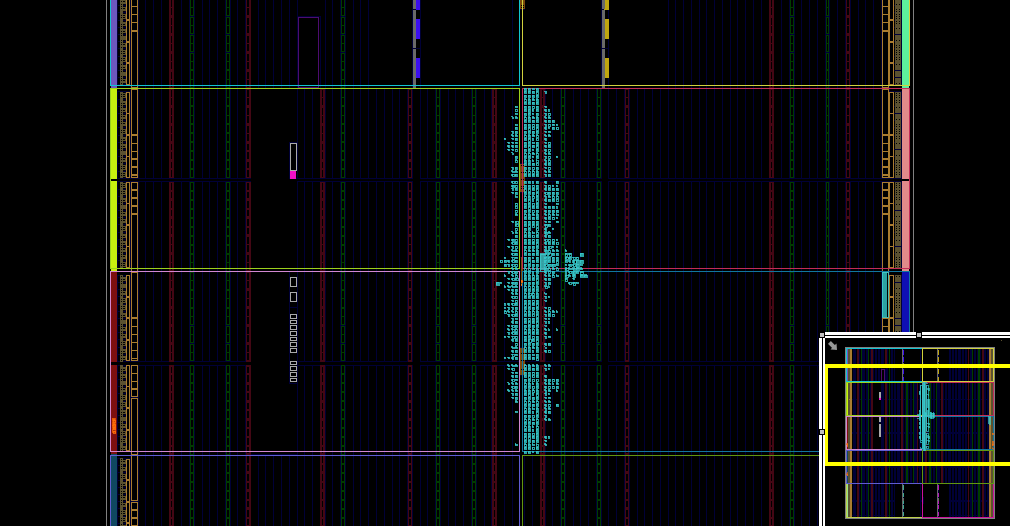
\includegraphics[width=0.8\textwidth]{imagenes/floorplan_0.png}
      \caption{Implementación del TDC en la Artix-7.}
      \label{fig: floorplan_0}
 \end{figure}

 \begin{figure}[H]
      \centering
      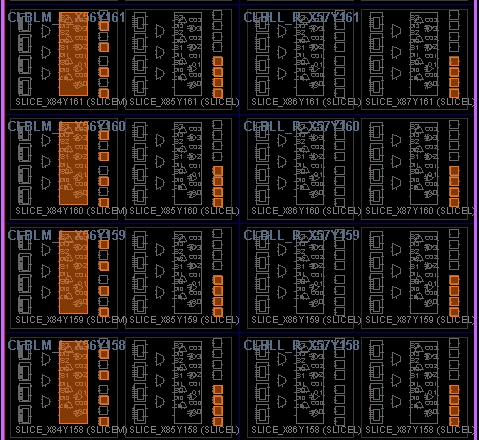
\includegraphics[width=0.75\textwidth]{imagenes/floorplan_carrys.png}
      \caption{A la izquierda el slice contiene cada Carry4 y su registro. Un Slice después se colocan
      los registros start, y dos slices después los registros stop, tal como en \cite{machado_novel_2018}.}
      \label{fig: floorplan_retardos}
 \end{figure}%
 \begin{figure}[H]
      \centering
      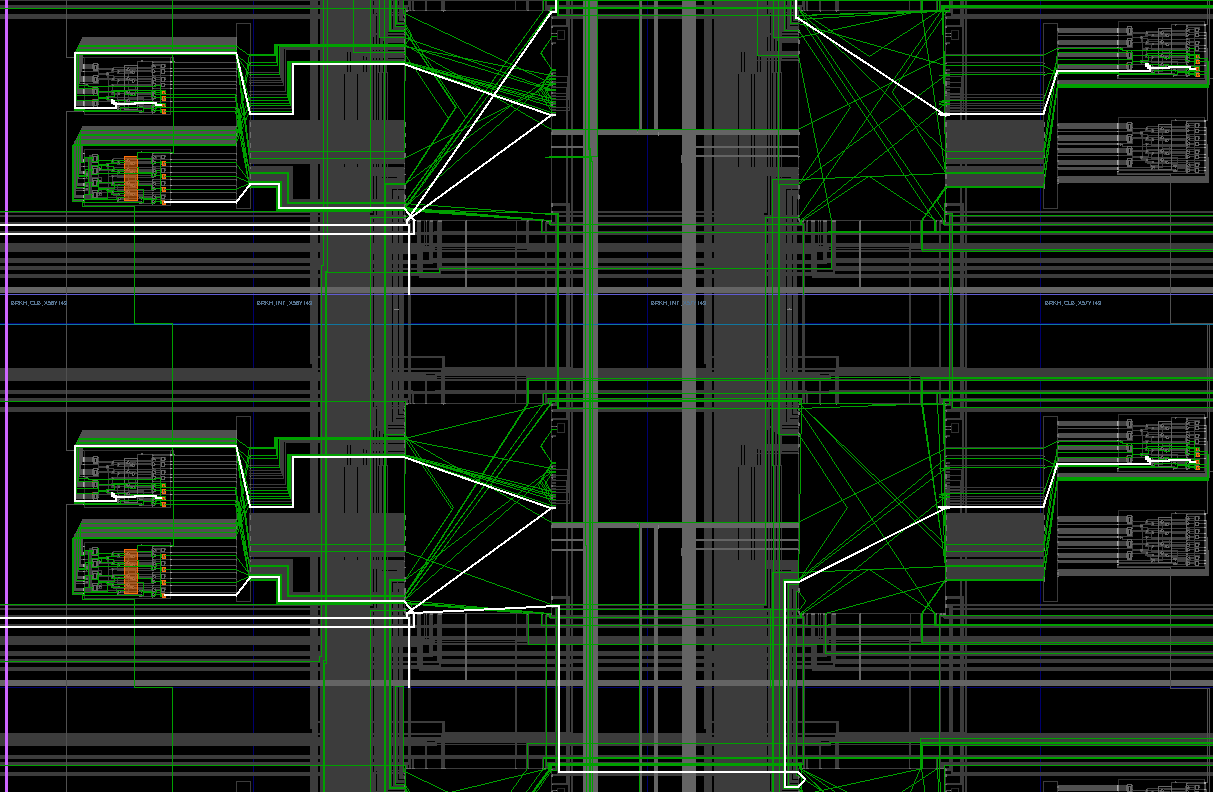
\includegraphics[width=0.75\textwidth]{imagenes/floorplan_routeo.png}
      \caption{Ruteo desde los retardos hacia sus registros.}
      \label{fig: ruteo}
 \end{figure}%
 \begin{figure}[H]
      \centering
      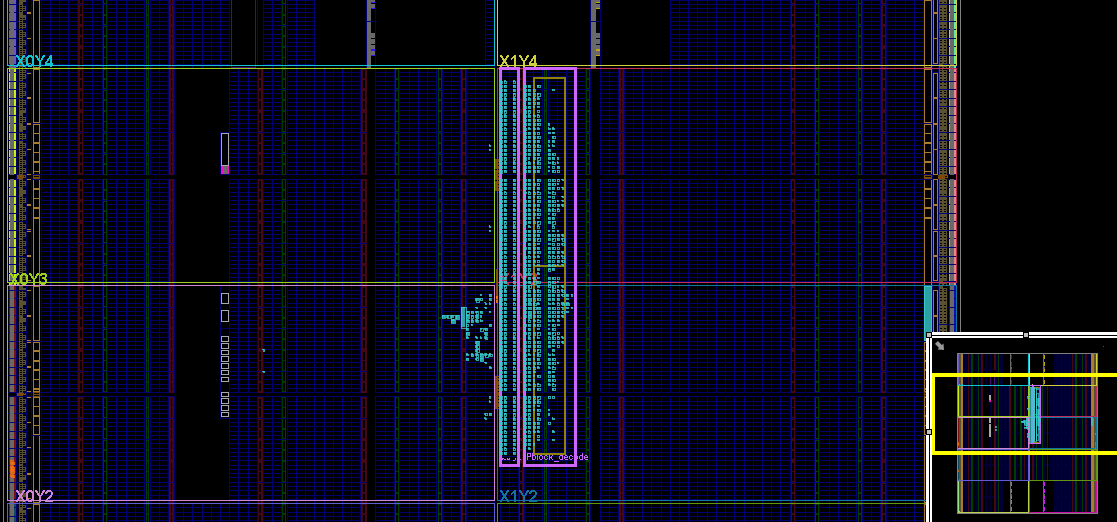
\includegraphics[width=0.75\textwidth]{imagenes/floorplan_pblocks.png}
      \caption{Esquema de distribución final. El primer rectángulo corresponde al \textit{P\_block} fino,
      y a su derecha el \textit{P\_block} para los decoders.}
      \label{fig: floorplan_pblocks}
 \end{figure}

 Con esta implementación, además se consiguió subir la frecuencia del sistema a $300$ MHz, de forma que se acortó 
 aún más el largo de la cadena. Las curvas de transferencia obtenidas son las que se muestran a continuación 
 en las Figuras \ref{fig: transferencia_start_med5}, \ref{fig: transferencia_stop_med5}

 \begin{figure}[H]
      \centering
      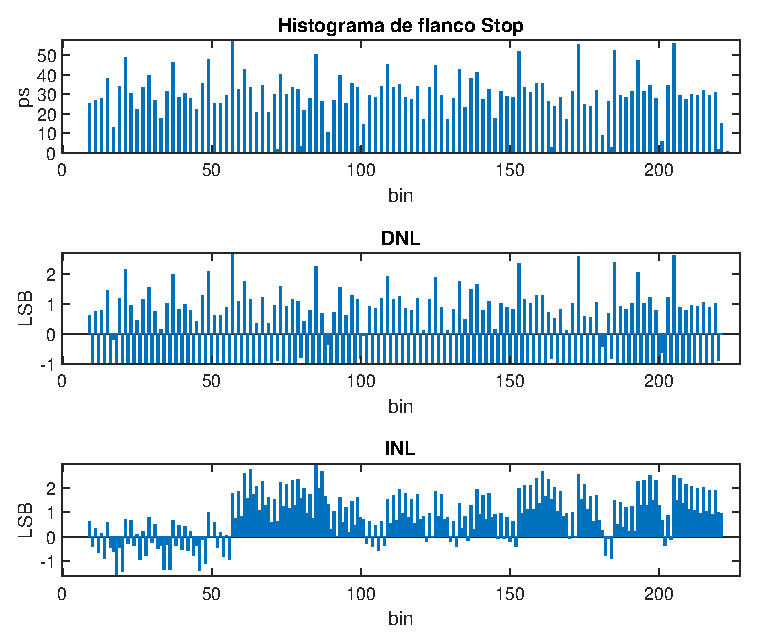
\includegraphics[width=0.75\textwidth]{imagenes/linealidad_stop_med5.eps}
      \caption{Histogramas de linealidad para la última implementación. Flanco stop.}
      \label{fig: transferencia_stop_med5}
 \end{figure}
 \begin{figure}[H]
     \centering
     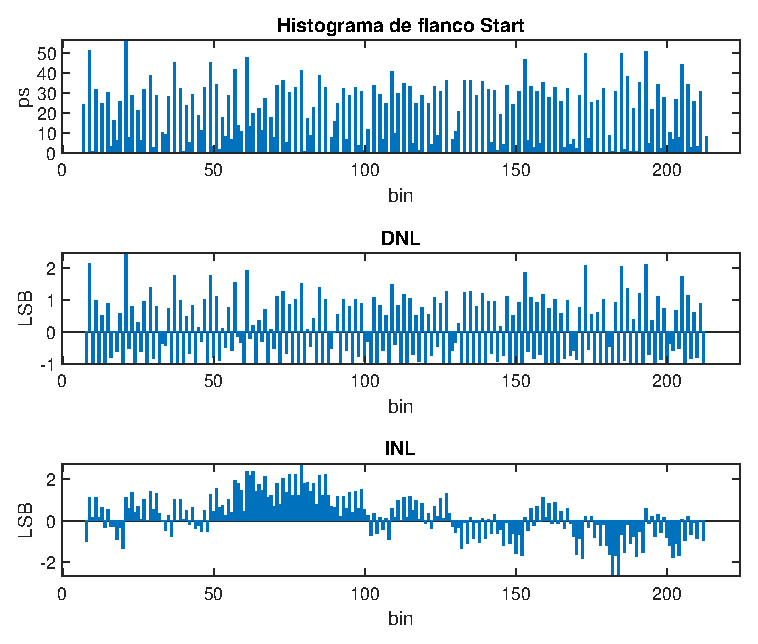
\includegraphics[width=0.75\textwidth]{imagenes/linealidad_start_med5.eps}
     \caption{Histogramas de linealidad para la última implementación. Flanco start.}
     \label{fig: transferencia_start_med5}
\end{figure}

Por último es posible implementar una calibración en memoria, de forma tal que la respuesta del TDC
tenga en cuenta las no linealidades obtenidas en la prueba de densidad de código. Con esto, la idea principal es
en vez de utilizar la Ecuación \ref{eq: t_fino}, guardar en una tabla la curva de transferencia obtenida
al realizar la calibración, de forma tal que el tiempo medido en el i-ésimo bin es,
\begin{equation*}
     t_i = \dfrac{\tau_i}{2} + \sum_{k=0}^{i-1} \tau_k \; ,
\end{equation*}
donde la definición de $\tau_i$ proviene de la Ecuación \ref{eq: tau_i}. \\
Tal como dice \textit{Wu} en \cite{Wu2010}, es muy fácil caer en sólo computar la sumatoria cuando
la implementación se vuelve engorrosa, pero sería un error omitir $\tau_i/2$ ya que esto implica calibrar
a la mitad del bin en vez de hacerlo a los bordes, lo que disminuye el error RMS al mínimo.

\subsection{Discusión}
Se ha medido con la calibración final propuesta en este trabajo, con lo que se ha conseguido mejorar
la precisión a valores de entre 19 ps y 17 ps (Figura \ref{fig: medicion_final}). Aún así no se ha logrado 
corregir el offset, que se ha mantenido en el mismo rango. Se han reportado sesgos de alrededor de 500ps,
utilizando la misma topología en \cite{machado_readout_2020}. \\

\begin{figure}[H]
      \centering
      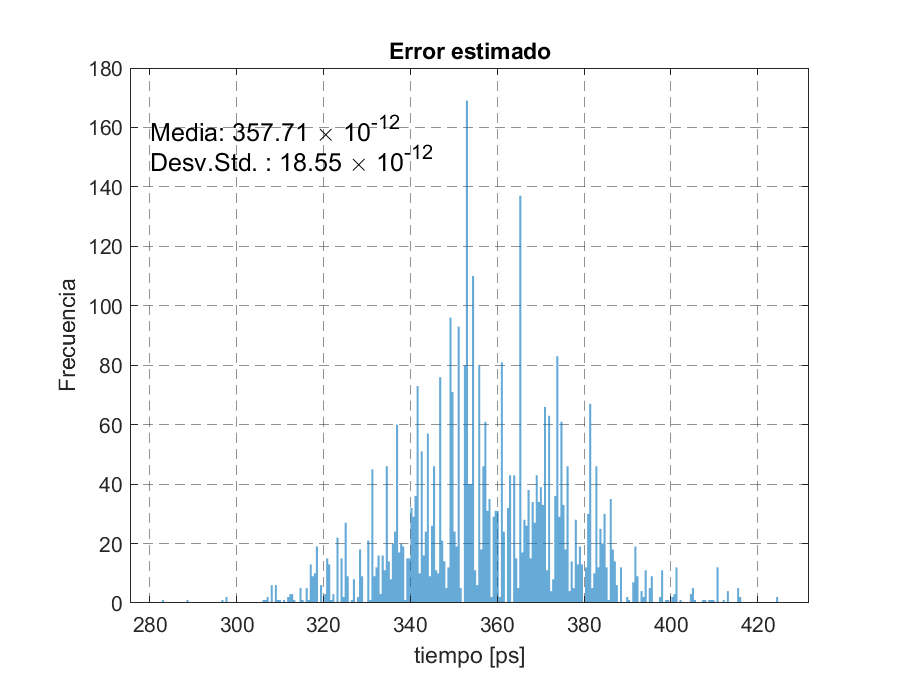
\includegraphics[width=0.75\textwidth]{imagenes/Medicion_final.eps}
      \caption{Error computado al realizar la diferencia de la media calculada y el semiperíodo 
      teórico $t_\text{on} = 15.15\;\mu$s, para 4096 mediciones con una señal de frecuencia $f=3.3M$Hz.}
      \label{fig: medicion_final}
\end{figure}

Para desambiguar, es necesario seguir trabajando en caracterizar
el buffer de entrada al ingresar la señal a través del estándar \textit{LVDS\_25}, y con esto conocer a ciencia
cierta la dinámica de la señal que se distribuye a través de la cadena, o en su defecto, realizar un circuito 
de acondicionamiento de forma tal que, conocida su transferencia, se pueda tener en cuenta dentro de la calibración
final.\\
A pesar de estos problemas, se ha logrado satisfactoriamente alcanzar una precisión del orden de la decena de picosegundos,
con lo cuál es posible utilizar esta implementación en las aplicaciones propuestas. Creemos que los horizontes de trabajo para futuras
implementaciones son:
\begin{itemize}
     \item Sincronización de la medición fina y gruesa.
     \item Auto-calibración en hardware.
     \item Comparativa con la implementación de un decodificador \textit{ones-counter}.
     \item Implementación multi-cadena.
\end{itemize}


    \clearpage
    \printbibliography[heading=bibintoc, title={Referencias}]


\end{document}
